\documentclass[12pt,a4paper]{article}

% --- Paket-paket Dasar ---
\usepackage[utf8]{inputenc}
\usepackage[indonesian]{babel}
\usepackage[T1]{fontenc}
\usepackage{geometry}
\geometry{top=3cm, bottom=3cm, left=3.5cm, right=2.5cm, headheight=15pt}

\usepackage{graphicx}
\usepackage{float}
\usepackage{caption}
\usepackage{subcaption}
\usepackage{booktabs}
\usepackage{tabularx}
\usepackage{longtable}
\usepackage{amsmath,amssymb}
\usepackage{listings}
\usepackage{xcolor}
\usepackage{fancyhdr}
\usepackage{titlesec}
\usepackage{enumitem}
\usepackage{tcolorbox}
\tcbuselibrary{skins,breakable}

% --- Deklarasi Dukungan Karakter Unicode untuk pdflatex ---
\DeclareUnicodeCharacter{2715}{\ensuremath{\times}}
\DeclareUnicodeCharacter{2713}{\ensuremath{\checkmark}}
\DeclareUnicodeCharacter{00B7}{\ensuremath{\cdot}}

\usepackage[hidelinks,colorlinks=true,linkcolor=blue!80!black,citecolor=blue,urlcolor=cyan!70!black]{hyperref}

% --- Konfigurasi Warna Neobrutalism ---
\definecolor{nbYellow}{RGB}{255, 212, 59}
\definecolor{nbRed}{RGB}{255, 122, 122}
\definecolor{nbCyan}{RGB}{122, 231, 247}
\definecolor{nbLime}{RGB}{185, 242, 124}
\definecolor{nbPurple}{RGB}{195, 166, 255}
\definecolor{nbInk}{RGB}{17, 17, 17}
\definecolor{nbPaper}{RGB}{255, 252, 242}
\definecolor{nbCream}{RGB}{255, 241, 201}
\definecolor{codeGray}{RGB}{245, 245, 245}

% --- Konfigurasi Listing Kode ---
\lstset{
    backgroundcolor=\color{codeGray},
    basicstyle=\ttfamily\footnotesize,
    breaklines=true,
    captionpos=b,
    commentstyle=\color{gray},
    keywordstyle=\color{blue}\bfseries,
    stringstyle=\color{orange!80!black},
    frame=single,
    rulecolor=\color{black},
    numbers=left,
    numberstyle=\tiny\color{gray},
    stepnumber=1,
    tabsize=2,
    showstringspaces=false
}

% --- Header & Footer ---
\pagestyle{fancy}
\fancyhf{}
\fancyhead[L]{\textsl{TUGAS UAS PEMROGRAMAN WEB 2 -- KLIKIN}}
\fancyhead[R]{\textsl{\thepage}}
\fancyfoot[C]{\footnotesize Dokumentasi Sistem Bio \& Affiliate Platform dengan Otoritas Master \& Fitur DO NOT CROSS}
\renewcommand{\headrulewidth}{0.8pt}
\renewcommand{\footrulewidth}{0.4pt}

\begin{document}

% ========================================================
% COVER / HALAMAN JUDUL
% ========================================================
\begin{titlepage}
    \hypersetup{pageanchor=false}
    \centering
    \vspace*{1.5cm}
    
    {\Huge \bfseries TUGAS AKHIR SEMESTER (UAS)\par}
    \vspace{0.4cm}
    {\LARGE \bfseries PEMROGRAMAN WEB 2\par}
    \vspace{1.2cm}
    
    \begin{tcolorbox}[
        colback=nbYellow,
        colframe=nbInk,
        boxrule=2.5pt,
        arc=0mm,
        width=0.95\textwidth,
        halign=center
    ]
        \vspace{0.3cm}
        {\LARGE \bfseries DOKUMENTASI SISTEM APLIKASI WEB ``KLIKIN''\par}
        \vspace{0.3cm}
        {\large Platform Bio Link \& Manajemen Affiliate Berbasis Multi-Role (Master \& User) dengan Sistem Keamanan Pembekuan Profil (DO NOT CROSS)\par}
        \vspace{0.2cm}
    \end{tcolorbox}
    
    \vspace{1.5cm}
    
    \begin{minipage}{\textwidth}
        \large
        \begin{tabularx}{\textwidth}{@{}p{3.5cm}p{0.3cm}X@{}}
            \textbf{Mata Kuliah} & : & Pemrograman Web 2 \\
            \textbf{Topik Proyek} & : & Pengembangan Web Fullstack Modern dengan Laravel \\
            \textbf{Fitur Utama} & : & Multi-Role Authority (Master \& User), Ban Management, DO NOT CROSS Violation Scene, Database Seeding, Automated Feature \& Unit Testing (Pest PHP) \\
            \textbf{Tahun Ajaran} & : & 2026 / 2027 \\
        \end{tabularx}
    \end{minipage}
    
    \vfill
    
    {\large \bfseries PROGRAM STUDI TEKNIK INFORMATIKA / SISTEM INFORMASI\par}
    {\large FAKULTAS ILMU KOMPUTER\par}
    \vspace{0.8cm}
    {\large 2026}
\end{titlepage}

\hypersetup{pageanchor=true}
\pagenumbering{roman}
\tableofcontents
\newpage
\listoffigures
\listoftables
\newpage
\pagenumbering{arabic}

% ========================================================
% BAB 1: PENDAHULUAN
% ========================================================
\section{Pendahuluan \& Gambaran Umum Aplikasi}

\subsection{Latar Belakang}
Dalam era digital marketing dan konten kreator saat ini, pemasaran afiliasi (\textit{affiliate marketing}) telah menjadi salah satu sumber pendapatan paling masif bagi kreator konten di media sosial (Instagram, TikTok, YouTube, X). Namun, para kreator sering kali menghadapi kendala keterbatasan ruang penempatan tautan di bio profil mereka, serta maraknya tautan penipuan (\textit{phishing} dan judi \textit{online}) yang dapat merugikan pengikut mereka.

Aplikasi web \textbf{KLIKIN} hadir sebagai solusi platform \textit{bio link} dan manajemen produk afiliasi yang modern, responsif, dan mengedepankan keamanan. Dengan KLIKIN, kreator dapat:
\begin{enumerate}[noitemsep]
    \item Mengelompokkan produk afiliasi per kategori (contoh: Gadget, Kecantikan, Rumah Tangga).
    \item Membagikan satu tautan publik personal (\texttt{/u/\{username\}}).
    \item Melacak jumlah klik dari tiap produk afiliasi secara \textit{real-time}.
\end{enumerate}

\subsection{Pengembangan Fitur Multi-Role \& Penegakan Aturan}
Sebelumnya, sistem belum memiliki tingkatan hak akses (\textit{role}) yang membedakan pengguna biasa dan pengelola platform. Untuk menjaga integritas ekosistem dari penyebaran tautan terlarang, penipuan, atau produk ilegal, dilakukan pembaharuan sistem berupa:
\begin{itemize}
    \item \textbf{Role Master}: Otoritas tertinggi (administrator) yang memiliki akses memantau seluruh pengguna dan memiliki hak eksklusif untuk menangguhkan (\textit{ban}) atau memulihkan (\textit{unban}) akun yang melanggar aturan.
    \item \textbf{Role User}: Pengguna umum/kreator yang dapat mengelola produk, kategori, dan profil pribadinya.
    \item \textbf{Halaman Pelanggaran DO NOT CROSS}: Apabila suatu akun terbukti melanggar pedoman komunitas dan di-\textit{ban} oleh Master, seluruh akses produk afiliasinya ditutup dan halaman publik profil kreator tersebut disegel dengan tampilan barikade garis polisi (\textit{Police Line / DO NOT CROSS}) bernuansa Neobrutalism yang mencolok beserta rincian alasan penindakan.
    \item \textbf{Seeder Otomatis}: Penyediaan seeder untuk membuat akun Master dan akun User (kreator aktif maupun contoh akun pelanggar ter-\textit{ban}) secara otomatis.
\end{itemize}

\subsection{Spesifikasi Teknologi (Tech Stack)}
Aplikasi ini dibangun menggunakan arsitektur web modern dengan rincian:
\begin{table}[H]
    \centering
    \caption{Spesifikasi Teknologi Aplikasi KLIKIN}
    \begin{tabularx}{\textwidth}{lX}
        \toprule
        \textbf{Komponen} & \textbf{Teknologi / Pustaka yang Digunakan} \\
        \midrule
        \textbf{Backend Framework} & Laravel 13 (PHP 8.5) \\
        \textbf{Database Engine} & SQLite / MySQL dengan ULID (\textit{Universally Unique Lexicographically Sortable Identifier}) \\
        \textbf{Frontend Styling} & Tailwind CSS v3.4 dengan tema Neobrutalism kustom (\textit{high-contrast borders}, \textit{hard shadow}, warna pop) \\
        \textbf{Frontend Reactivity} & Alpine.js v3 \& Blade Templating Engine \\
        \textbf{Asset Bundler} & Vite v8 \\
        \textbf{Testing Framework} & Pest PHP 5 (Feature \& Unit Testing) \\
        \textbf{Autentikasi} & Laravel Breeze dengan Custom Multi-Role Middleware \\
        \bottomrule
    \end{tabularx}
\end{table}

\newpage

% ========================================================
% BAB 2: SISTEM OTORITAS & KEBIJAKAN KEAMANAN
% ========================================================
\section{Sistem Otoritas, Peran (Roles), \& Fitur Keamanan}

\subsection{Matriks Hak Akses (Access Control Matrix)}
Sistem menerapkan pembagian hak akses yang ketat antara akun tamu (\textit{guest}), kreator (\textit{user}), dan pengelola (\textit{master}):

\begin{table}[H]
    \centering
    \small
    \caption{Matriks Hak Akses Berdasarkan Role}
    \begin{tabularx}{\textwidth}{>{\raggedright\arraybackslash}Xcccc}
        \toprule
        \textbf{Aktivitas / Fitur} & \textbf{Guest} & \textbf{User Aktif} & \textbf{User Banned} & \textbf{Master} \\
        \midrule
        Melihat Halaman Landing & $\checkmark$ & $\checkmark$ & $\checkmark$ & $\checkmark$ \\
        Mendaftar Akun Baru & $\checkmark$ & -- & -- & -- \\
        Masuk / Login ke Akun & $\checkmark$ & $\checkmark$ & $\times$ (Ditolak) & $\checkmark$ \\
        Mengakses Dashboard Pribadi & $\times$ & $\checkmark$ & $\times$ (Logout) & $\checkmark$ \\
        Mengelola Produk \& Kategori & $\times$ & $\checkmark$ & $\times$ & $\checkmark$ \\
        Melihat Profil Publik Aktif & $\checkmark$ & $\checkmark$ & $\checkmark$ & $\checkmark$ \\
        Melihat Profil Banned & Barikade & Barikade & Barikade & Barikade + Unban \\
        Klik Redirect Produk Affiliate & $\checkmark$ & $\checkmark$ & $\times$ (403 Block) & $\checkmark$ \\
        Mengakses Panel Pengguna & $\times$ & $\times$ (403) & $\times$ (403) & $\checkmark$ \\
        Melakukan Tindakan Ban & $\times$ & $\times$ & $\times$ & $\checkmark$ \\
        Melakukan Tindakan Unban & $\times$ & $\times$ & $\times$ & $\checkmark$ \\
        \bottomrule
    \end{tabularx}
\end{table}

\subsection{Arsitektur Penegakan Aturan (Ban System)}
Atribut penegakan aturan disimpan pada tabel \texttt{users} melalui migrasi:
\begin{itemize}[noitemsep]
    \item \texttt{role}: Bertipe \texttt{string}, nilai default \texttt{'user'}. Bernilai \texttt{'master'} untuk administrator.
    \item \texttt{is\_banned}: Bertipe \texttt{boolean}, default \texttt{false}.
    \item \texttt{banned\_at}: Bertipe \texttt{timestamp}, mencatat waktu penindakan.
    \item \texttt{ban\_reason}: Bertipe \texttt{text}, mencatat alasan spesifik penindakan oleh Master.
\end{itemize}

Penegakan keamanan diimplementasikan pada beberapa lapis (\textit{defense-in-depth}):
\begin{enumerate}
    \item \textbf{Middleware \texttt{EnsureUserIsMaster}}: Memvalidasi bahwa hanya pengguna dengan \texttt{\$user->isMaster() === true} yang diizinkan mengakses rute prefiks \texttt{/admin/*}. Pengguna tanpa wewenang akan langsung mendapatkan respon HTTP \texttt{403 Forbidden}.
    \item \textbf{Middleware \texttt{EnsureUserNotBanned}}: Terdaftar pada grup middleware global \texttt{'web'}. Apabila sesi pengguna yang sedang aktif dikenakan ban, middleware ini secara otomatis memutus sesi (\textit{logout}), menginvalidasi token sesi, dan mengarahkan ke halaman login dengan pesan peringatan pelanggaran.
    \item \textbf{Lapis Autentikasi \texttt{LoginRequest}}: Saat pengguna mencoba melakukan login, sistem memeriksa status akun. Jika akun ditandai \texttt{is\_banned}, kredensial ditolak dengan pesan kesalahan eksplisit yang menyertakan alasan ban.
    \item \textbf{Lapis Redirect Affiliate \texttt{AffiliateProductController@redirect}}: Menolak pengalihan URL sponsor jika kreator pemilik produk berstatus ter-\textit{ban}, guna melindungi masyarakat dari tautan berbahaya.
\end{enumerate}

\subsection{Konsep Visual Halaman Peringatan ``DO NOT CROSS''}
Sesuai dengan spesifikasi, profil kreator yang melanggar aturan tidak lagi menampilkan katalog produk, melainkan digantikan dengan halaman barikade garis polisi (\textit{Police Line DO NOT CROSS}) dengan karakteristik Neobrutalism:
\begin{itemize}[noitemsep]
    \item Pita bahaya miring (\textit{hazard stripes}) berwarna kuning dan hitam berulang-ulang di bagian atas, tengah, dan bawah halaman.
    \item Pita diagonal bertuliskan: \texttt{DO NOT CROSS // POLICE LINE // DO NOT CROSS}.
    \item Foto profil kreator dibuat monokrom (\textit{grayscale}) dengan stempel merah bertuliskan \texttt{BANNED [X]}.
    \item Kotak notifikasi resmi yang memuat tanggal penindakan serta alasan penindakan secara transparan.
    \item Apabila Master melihat halaman ini, tersedia \textit{Master Action Bar} di bagian teratas untuk memulihkan (\textit{unban}) pengguna tersebut secara instan.
\end{itemize}

\newpage

% ========================================================
% BAB 3: PENGELOLAAN DATABASE & SEEDER
% ========================================================
\section{Pengelolaan Database \& Seeder}

\subsection{Migrasi Database}
Pengembangan fitur ini menambahkan satu berkas migrasi baru yaitu:
\texttt{database/migrations/2026\_11\_11\_114535\_add\_role\_and\_ban\_fields\_to\_users\_table.php}.

\begin{lstlisting}[language=PHP, caption={Cuplikan Skema Migrasi Penambahan Kolom Role dan Ban}]
Schema::table('users', function (Blueprint $table) {
    $table->string('role')->default('user')->after('password');
    $table->boolean('is_banned')->default(false)->after('role');
    $table->timestamp('banned_at')->nullable()->after('is_banned');
    $table->text('ban_reason')->nullable()->after('banned_at');
});
\end{lstlisting}

\subsection{Implementasi Model User}
Pada model \texttt{App\textbackslash Models\textbackslash User}, ditambahkan metode penolong (\textit{helper methods}) yang menjamin kode bersih dan mudah dibaca:
\begin{lstlisting}[language=PHP, caption={Metode Helper pada Model User}]
public function isMaster(): bool
{
    return $this->role === 'master';
}

public function isUser(): bool
{
    return $this->role === 'user';
}

public function isBanned(): bool
{
    return (bool) $this->is_banned;
}

public function ban(?string $reason = null): void
{
    $this->update([
        'is_banned' => true,
        'banned_at' => now(),
        'ban_reason' => $reason,
    ]);
}

public function unban(): void
{
    $this->update([
        'is_banned' => false,
        'banned_at' => null,
        'ban_reason' => null,
    ]);
}
\end{lstlisting}

\subsection{Dokumentasi Seeder (Master \& User)}
Sesuai instruksi, dibuat dua berkas seeder khusus yang terpisah dan terorganisir dengan rapi:

\subsubsection{MasterSeeder (\texttt{database/seeders/MasterSeeder.php})}
Seeder ini bertugas menginisialisasi akun Master Administrator:
\begin{itemize}[noitemsep]
    \item \textbf{Nama}: Master Administrator
    \item \textbf{Username}: \texttt{master}
    \item \textbf{Email}: \texttt{master@klikin.id}
    \item \textbf{Password}: \texttt{password}
    \item \textbf{Role}: \texttt{master}
    \item \textbf{Bio}: Akun resmi Master Administrator KLIKIN. Mengawasi ketertiban, keamanan platform, dan berhak melakukan penangguhan terhadap pelanggar aturan.
\end{itemize}

\subsubsection{UserSeeder (\texttt{database/seeders/UserSeeder.php})}
Seeder ini menginisialisasi ekosistem pengguna reguler:
\begin{enumerate}
    \item \textbf{Demo Creator} (\texttt{demo@example.com} / \texttt{demo}): Akun kreator aktif dengan 3 kategori (Gadget, Kecantikan, Rumah Tangga) dan 7 produk afiliasi riil beserta jumlah klik awal.
    \item \textbf{Budi Santoso} (\texttt{budi@example.com} / \texttt{budisantoso}): Akun kreator aktif kategori Buku \& Edukasi.
    \item \textbf{Spammer Nakal} (\texttt{violator@example.com} / \texttt{violator}): Akun contoh yang telah di-\textit{ban} oleh Master dengan alasan \textit{``Melanggar Ketentuan Layanan: Memasang tautan affiliate phising dan penipuan undian palsu.''} Akun ini digunakan untuk mendemonstrasikan tampilan \textbf{DO NOT CROSS} secara nyata.
\end{enumerate}

Eksekusi seeder dilakukan melalui perintah:
\begin{lstlisting}[language=bash]
php artisan db:seed
\end{lstlisting}

\newpage

% ========================================================
% BAB 4: DOKUMENTASI LENGKAP FITUR & SCREENSHOT
% ========================================================
\section{Dokumentasi Fitur Aplikasi \& Tangkapan Layar (Screenshots)}

Berikut adalah dokumentasi komprehensif dari setiap fitur yang ada di dalam aplikasi web KLIKIN disertai tangkapan layar (\textit{screenshots}) langsung dari sistem yang sedang berjalan.

\subsection{Halaman Utama (Landing Page)}
Halaman pembuka yang menyambut pengunjung dengan visual Neobrutalism yang atraktif. Menjelaskan nilai utama aplikasi, tautan untuk mendaftar secara gratis, dan tombol demonstrasi profil publik.
\begin{figure}[H]
    \centering
    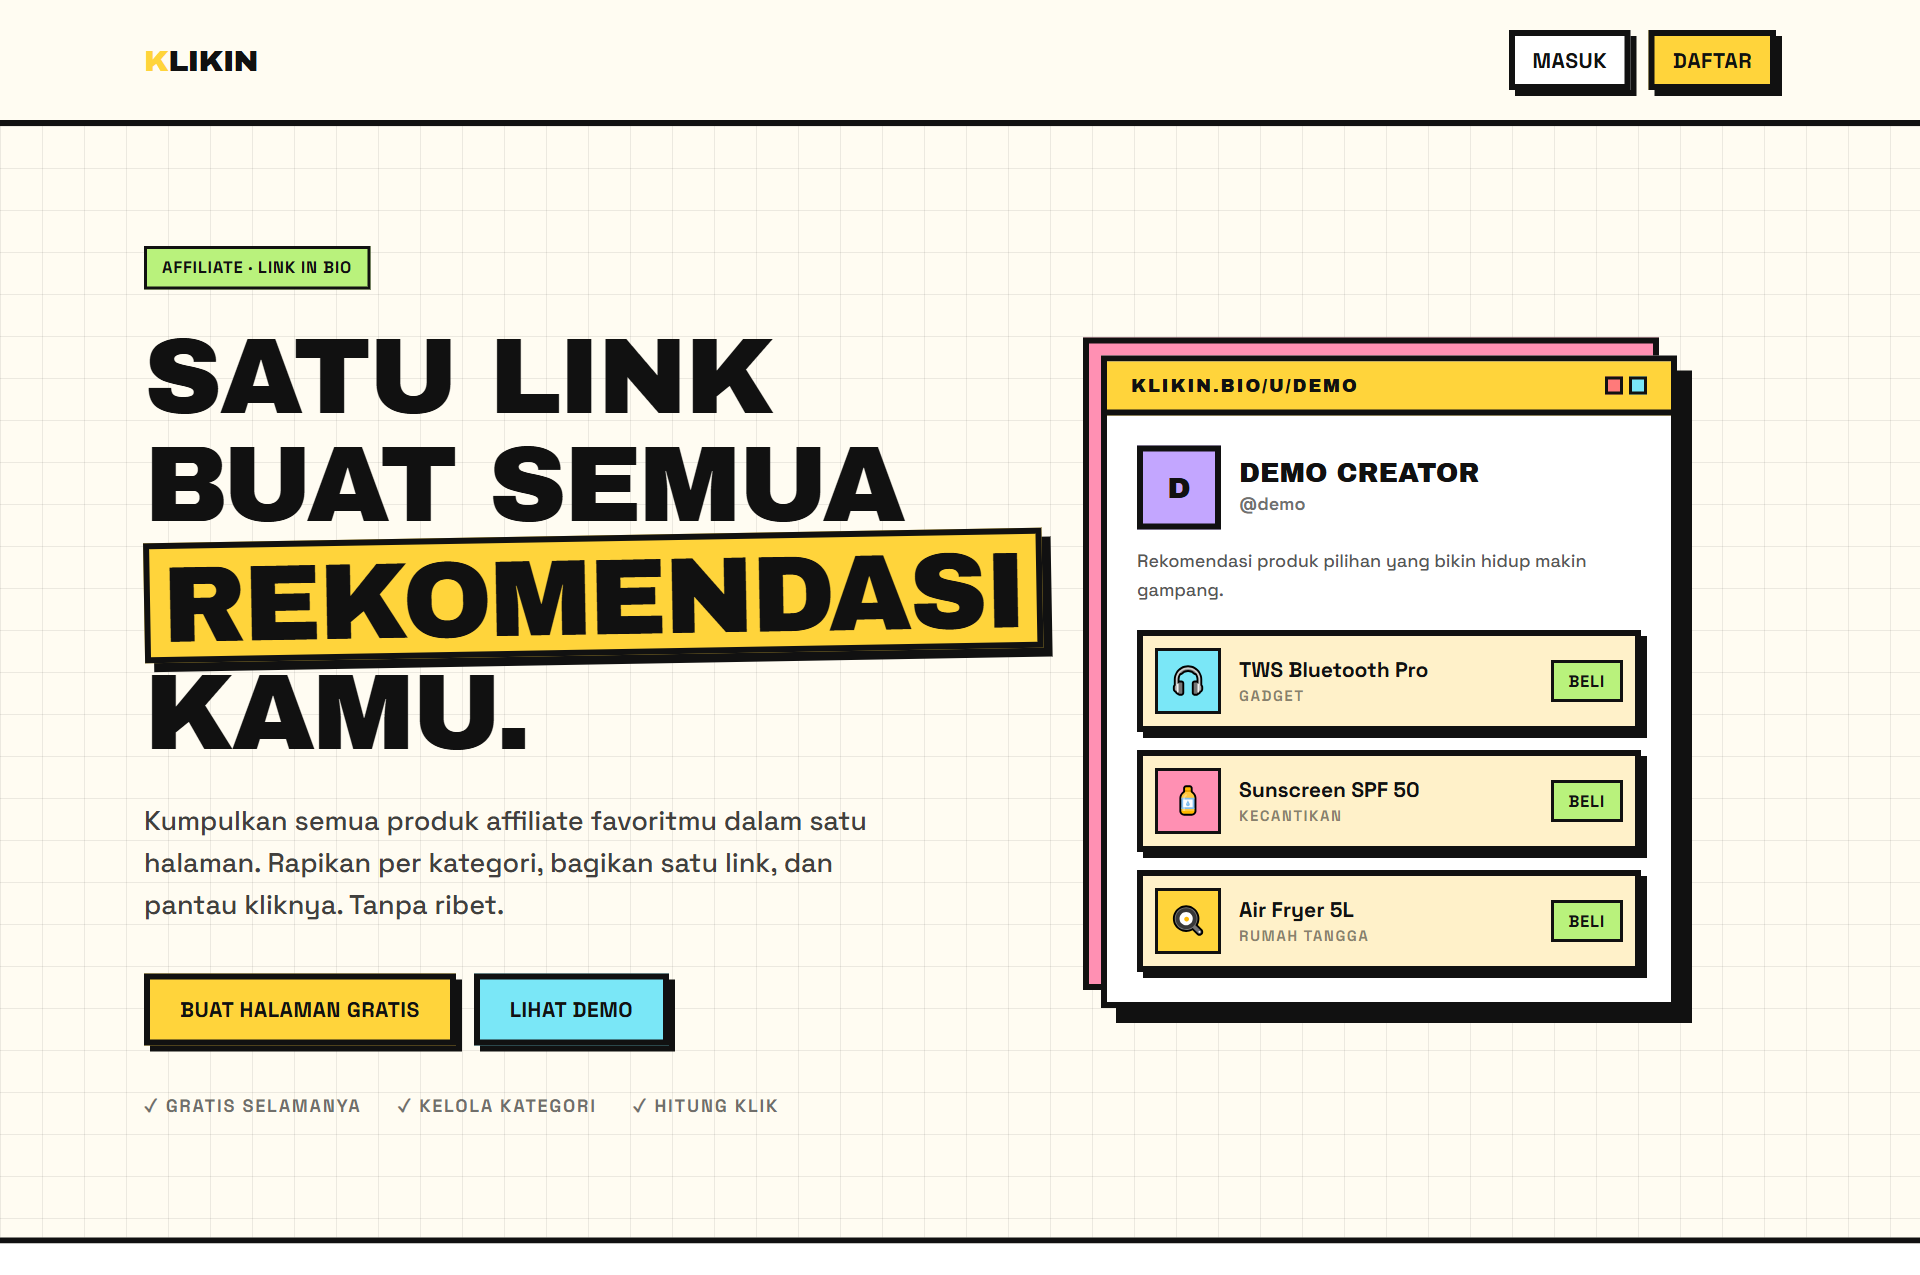
\includegraphics[width=0.92\textwidth]{images/01_landing_page.png}
    \caption{Halaman Utama (Landing Page) KLIKIN}
    \label{fig:landing}
\end{figure}

\subsection{Autentikasi Pengguna (Login \& Register)}
Sistem otentikasi dilengkapi dengan validasi ketat, perlindungan CSRF, dan pembatasan laju percobaan (\textit{rate limiting}).
\begin{figure}[H]
    \centering
    \begin{subfigure}[b]{0.48\textwidth}
        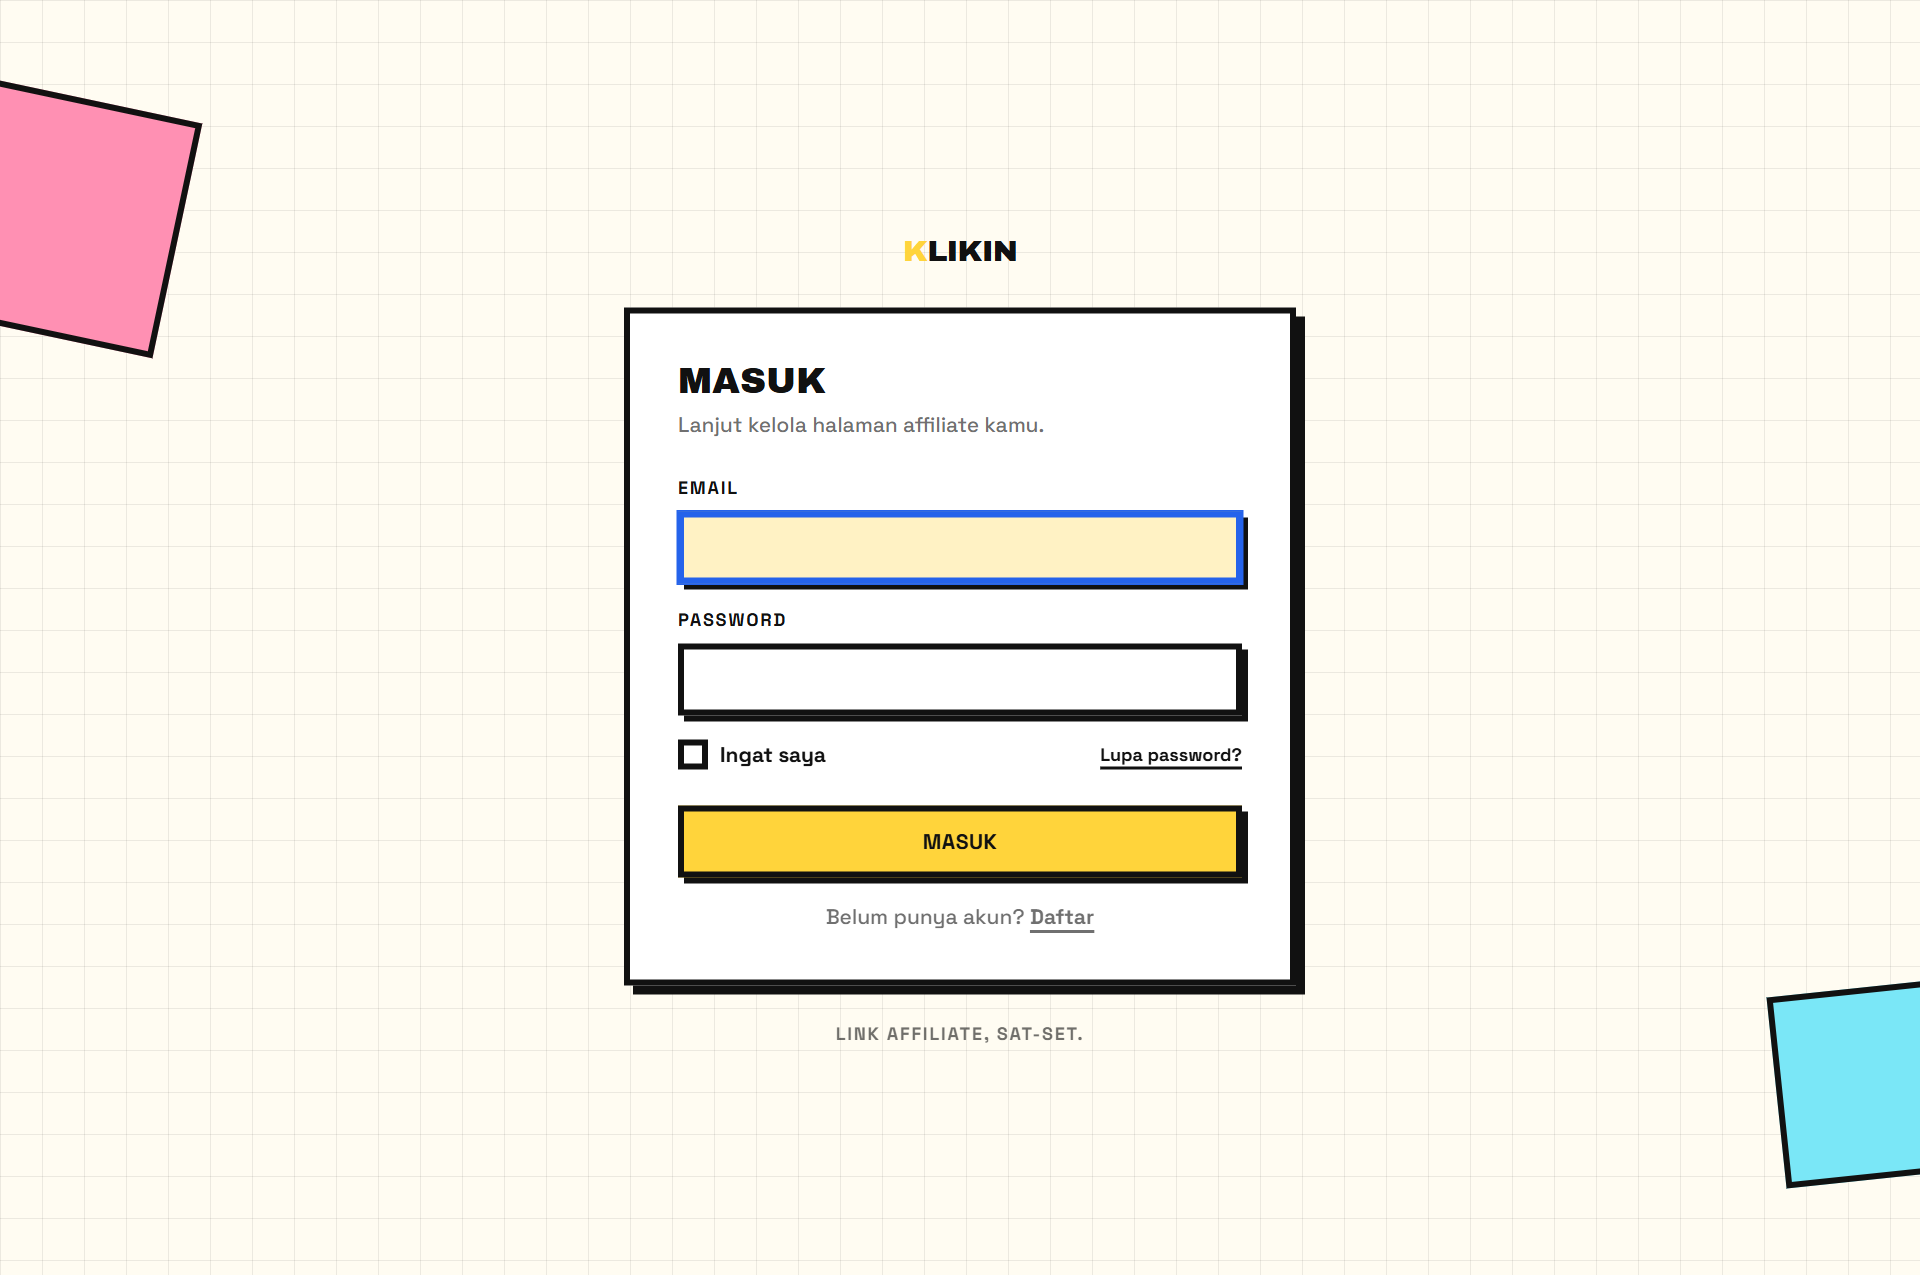
\includegraphics[width=\textwidth]{images/02_login_page.png}
        \caption{Halaman Masuk (Login)}
    \end{subfigure}
    \hfill
    \begin{subfigure}[b]{0.48\textwidth}
        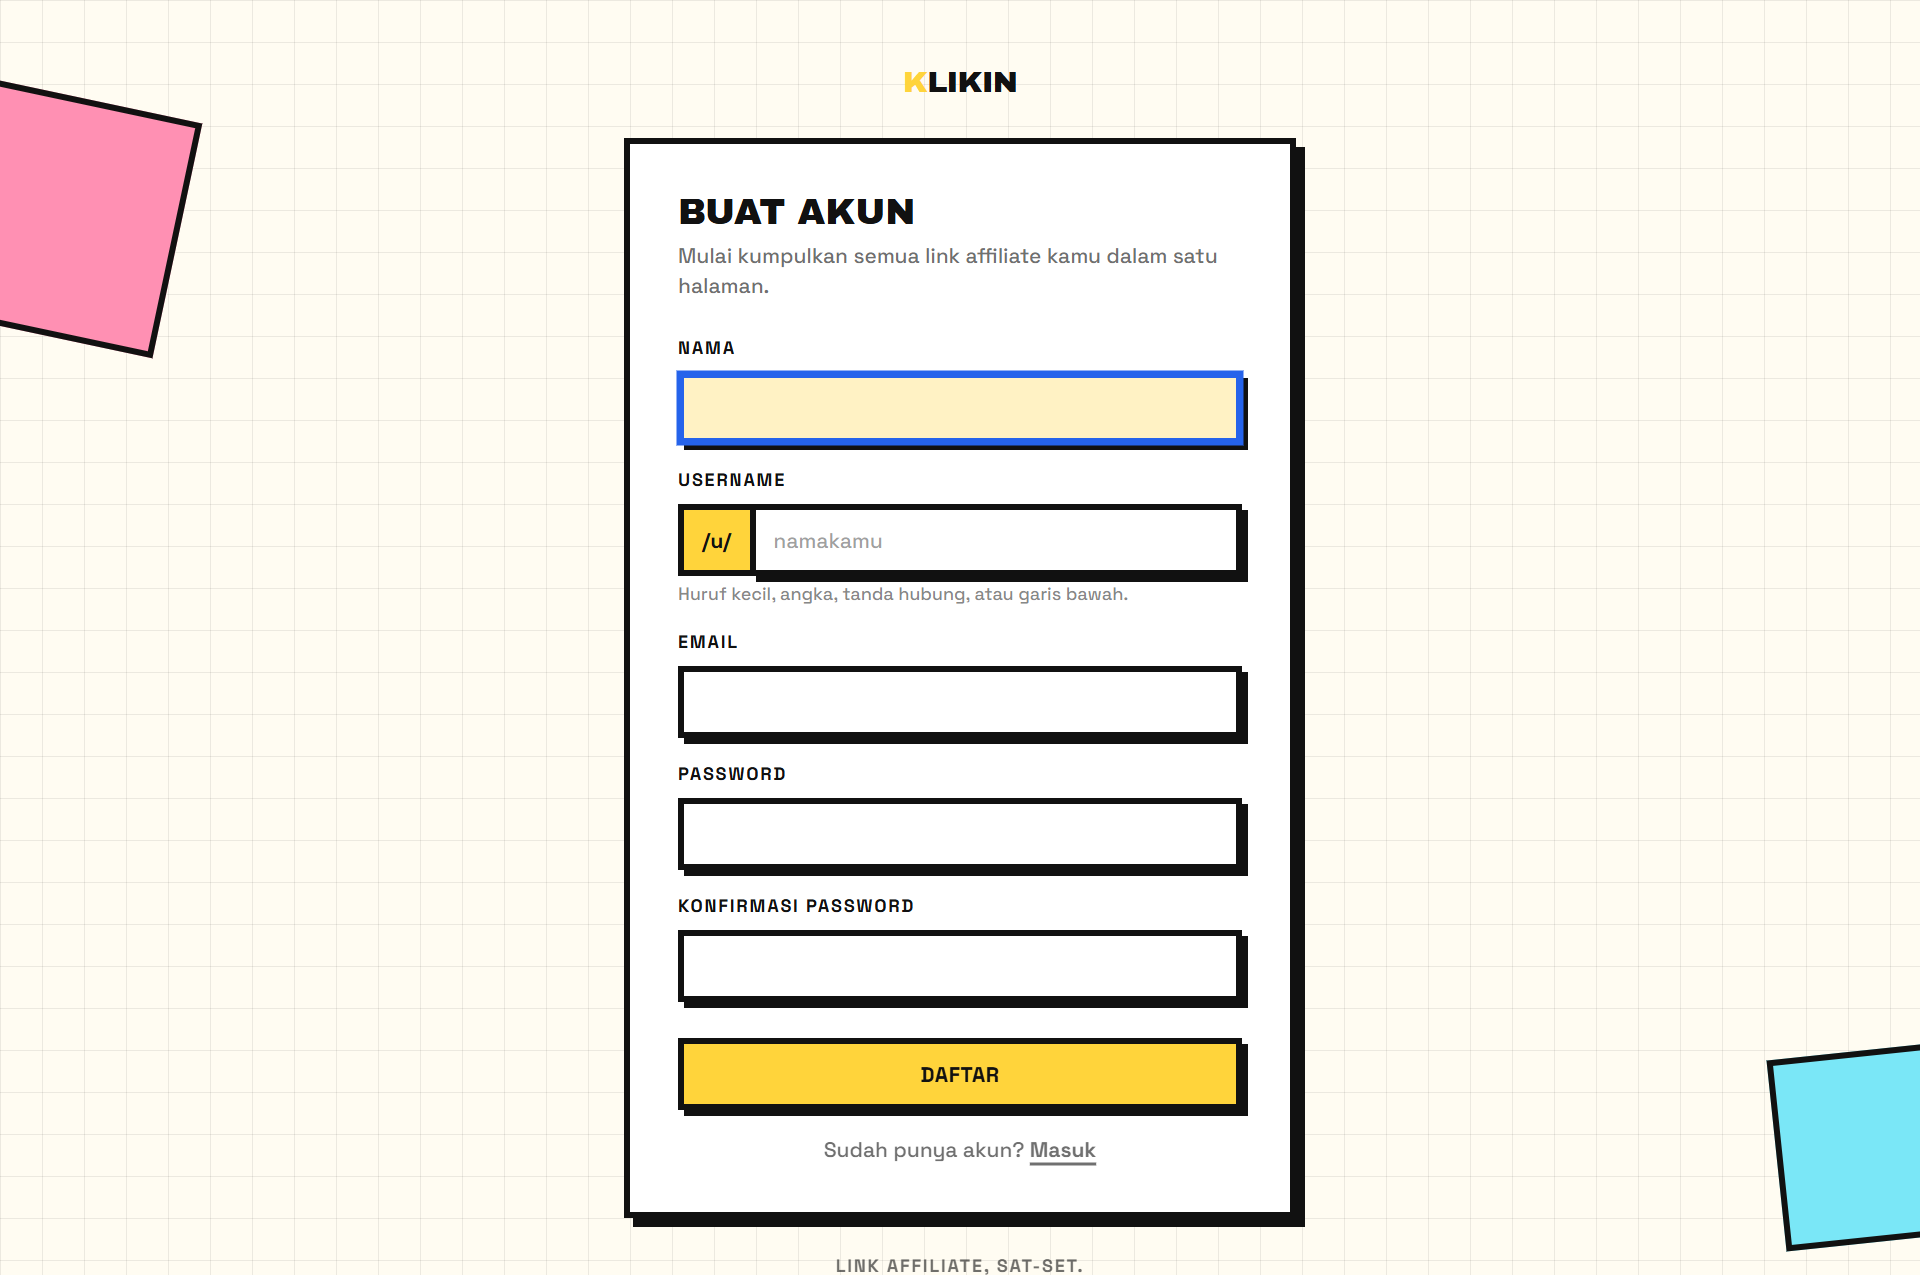
\includegraphics[width=\textwidth]{images/03_register_page.png}
        \caption{Halaman Pendaftaran (Register)}
    \end{subfigure}
    \caption{Antarmuka Masuk dan Pendaftaran Pengguna}
    \label{fig:auth}
\end{figure}

\newpage
\subsection{Dashboard Kreator / Pengguna}
Dashboard kreator menyajikan ringkasan metrik statistik seperti Total Produk, Total Kategori, dan Total Akumulasi Klik. Kreator juga dapat menyalin tautan publik bio miliknya dengan satu klik.
\begin{figure}[H]
    \centering
    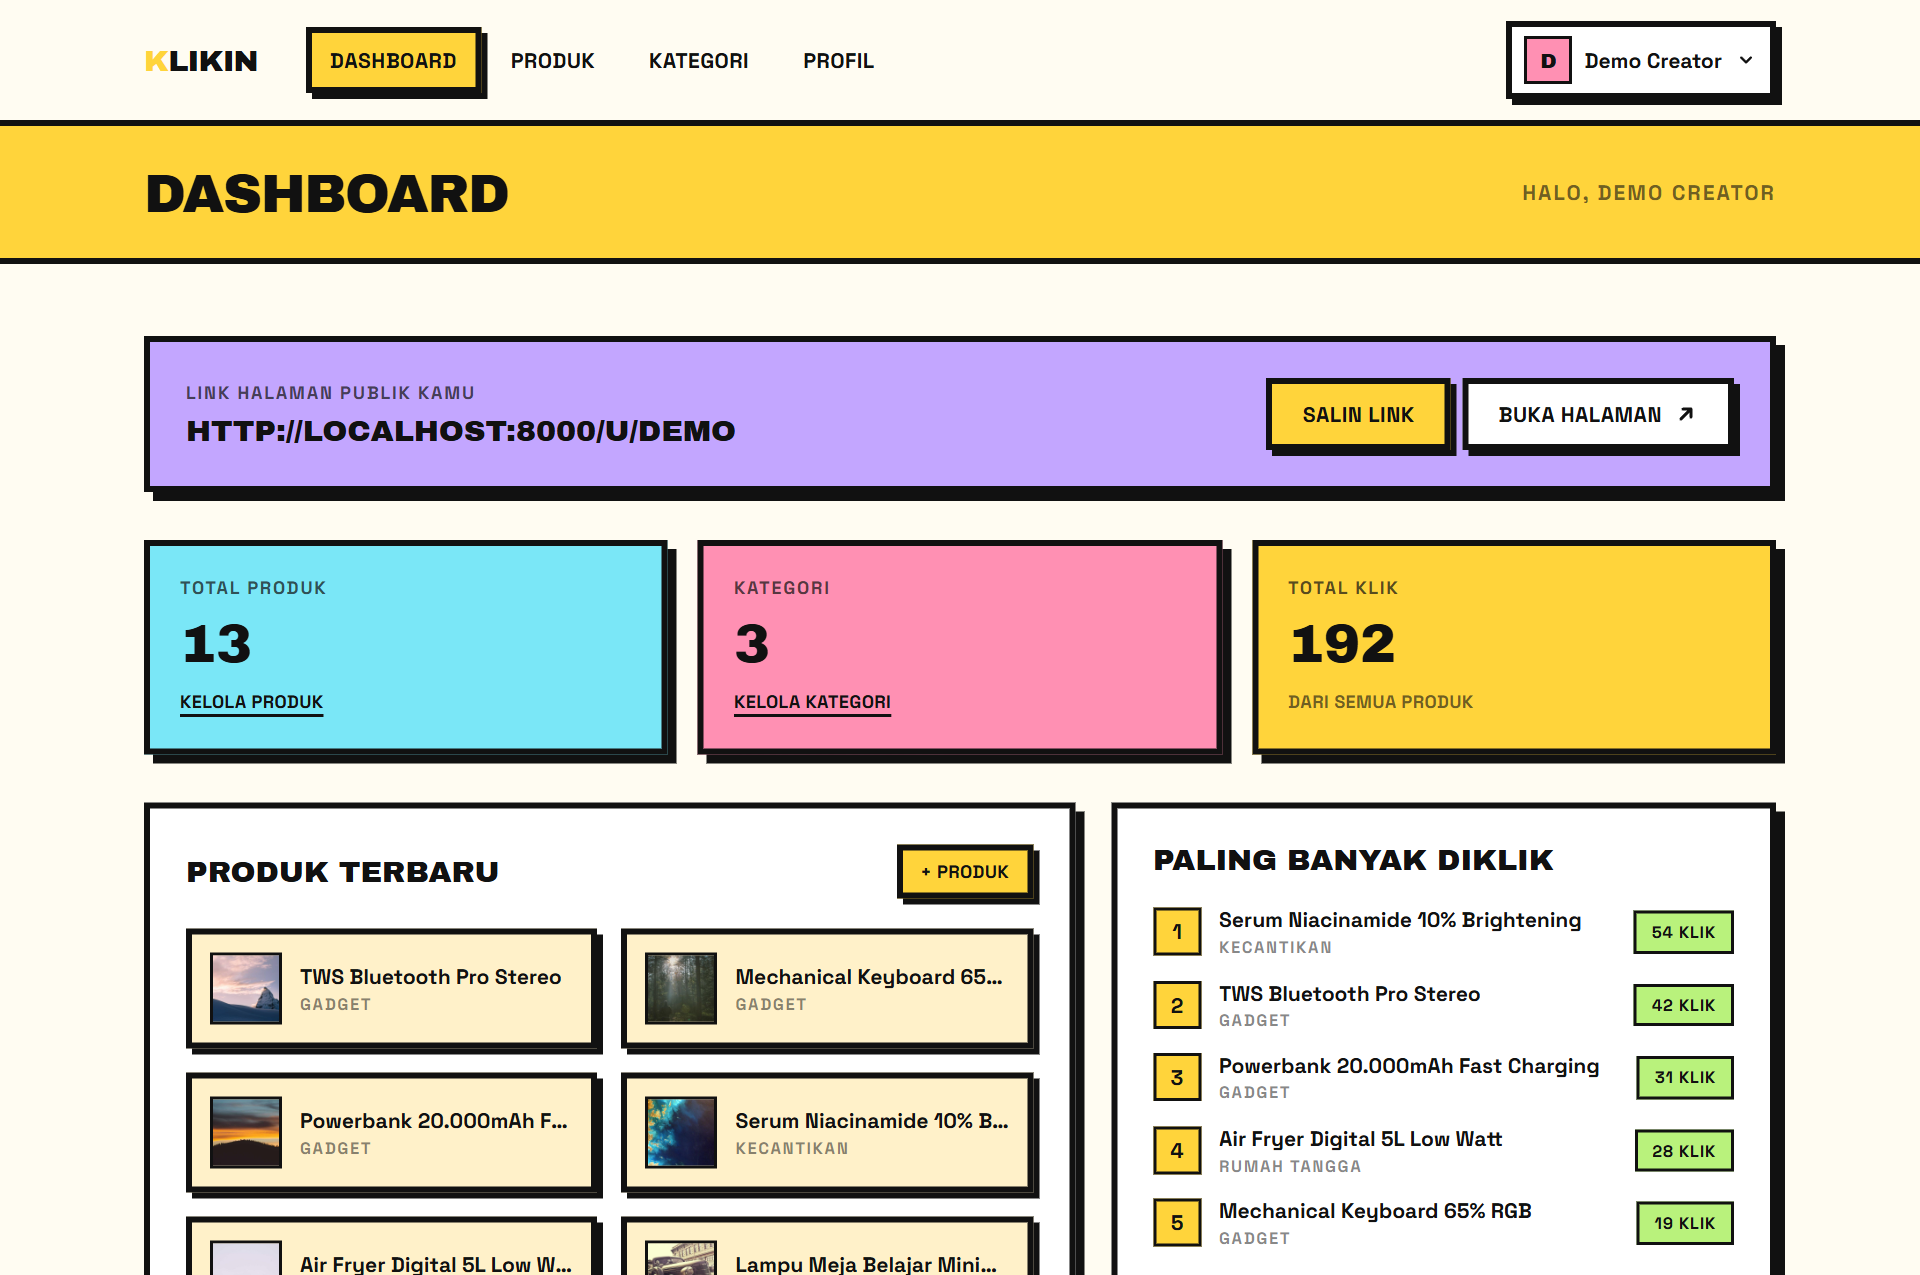
\includegraphics[width=0.92\textwidth]{images/04_user_dashboard.png}
    \caption{Dashboard Kreator (Role: User)}
    \label{fig:user_dashboard}
\end{figure}

\subsection{Manajemen Produk Afiliasi}
Kreator memiliki kendali penuh untuk melihat daftar produk afiliasi, mencari produk, menambah produk baru, menyunting, dan menghapus produk.
\begin{figure}[H]
    \centering
    \begin{subfigure}[b]{0.48\textwidth}
        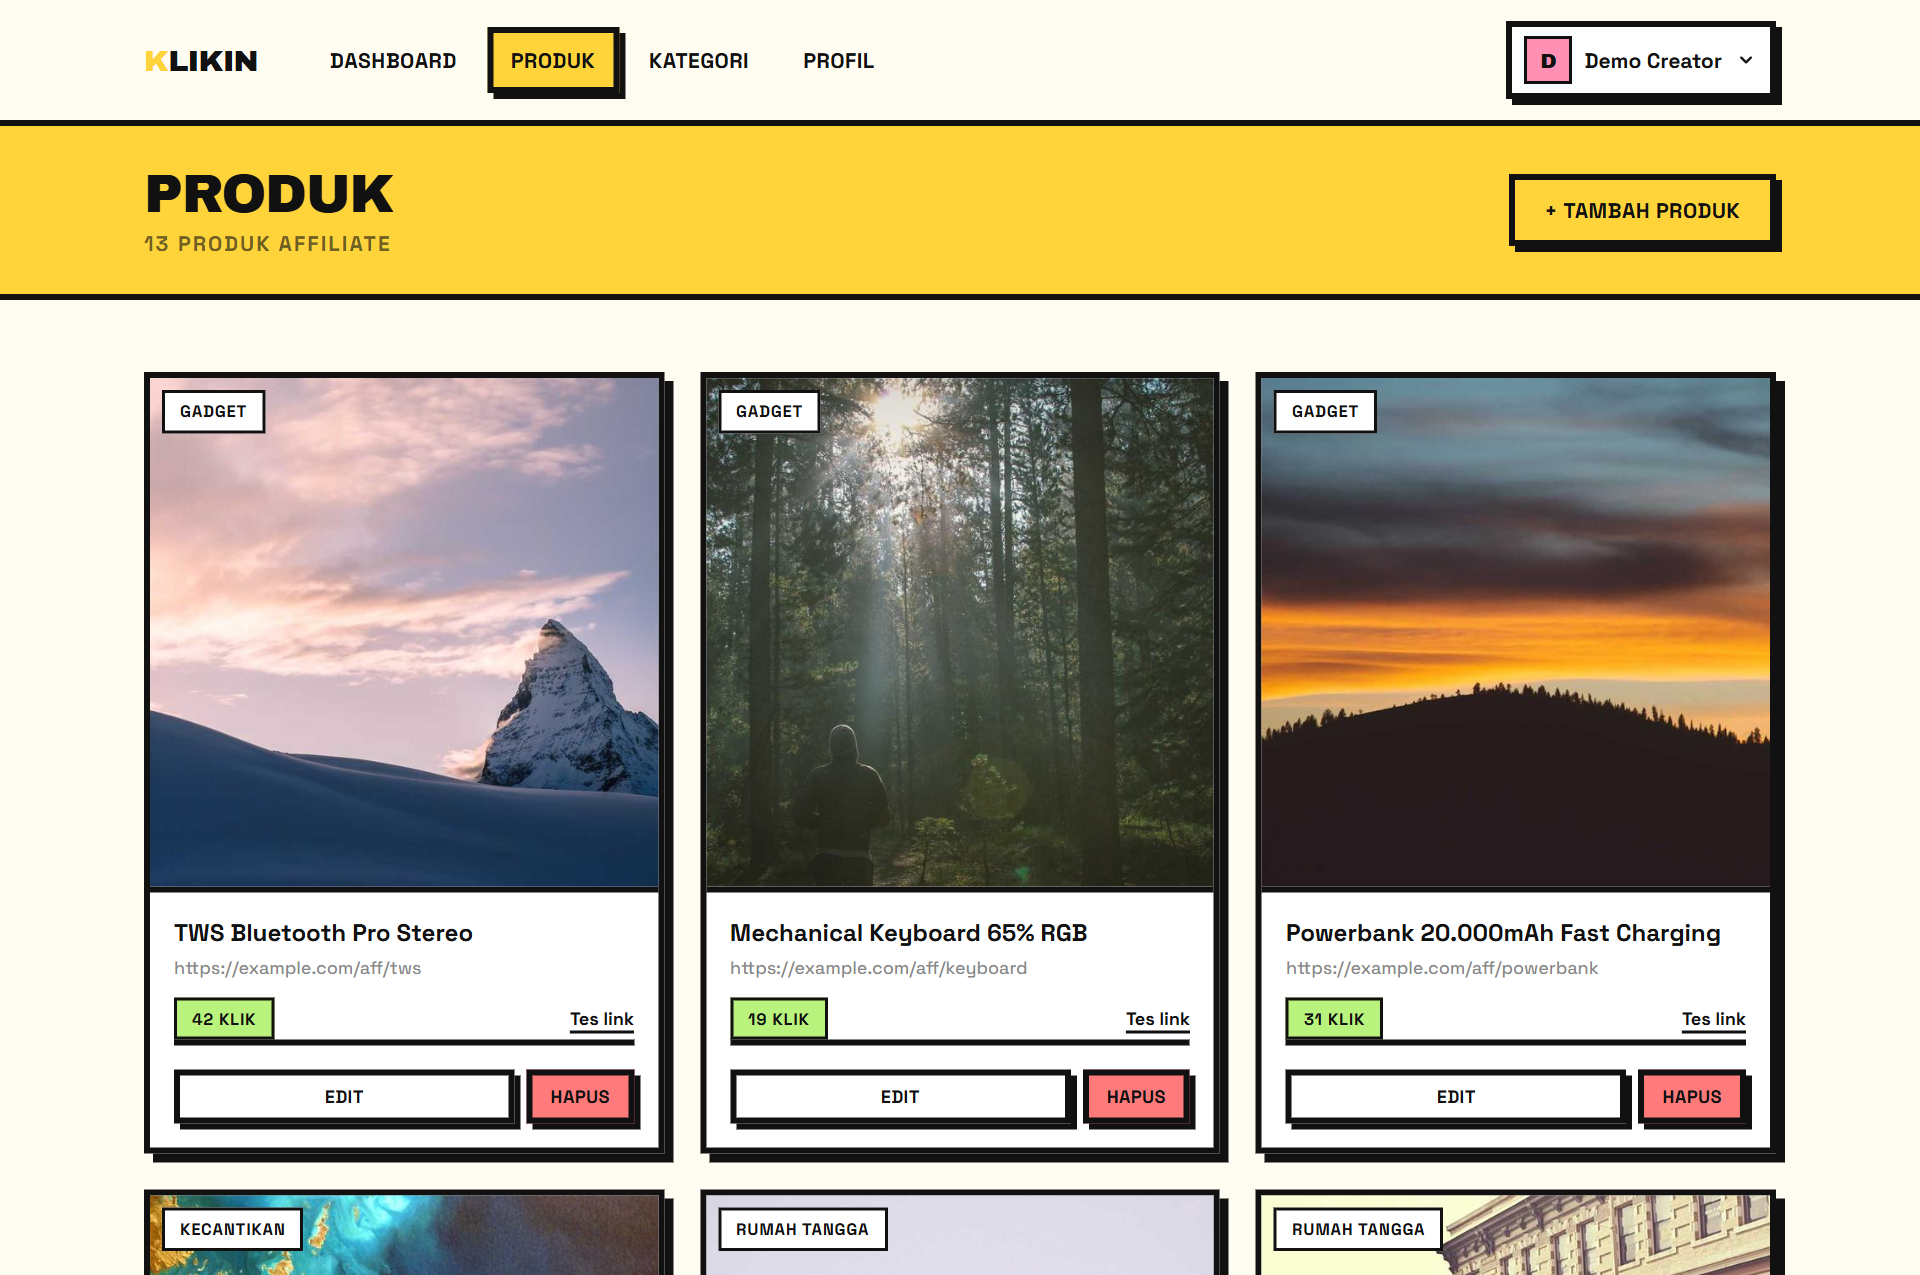
\includegraphics[width=\textwidth]{images/05_user_products.png}
        \caption{Daftar Katalog Produk Afiliasi}
    \end{subfigure}
    \hfill
    \begin{subfigure}[b]{0.48\textwidth}
        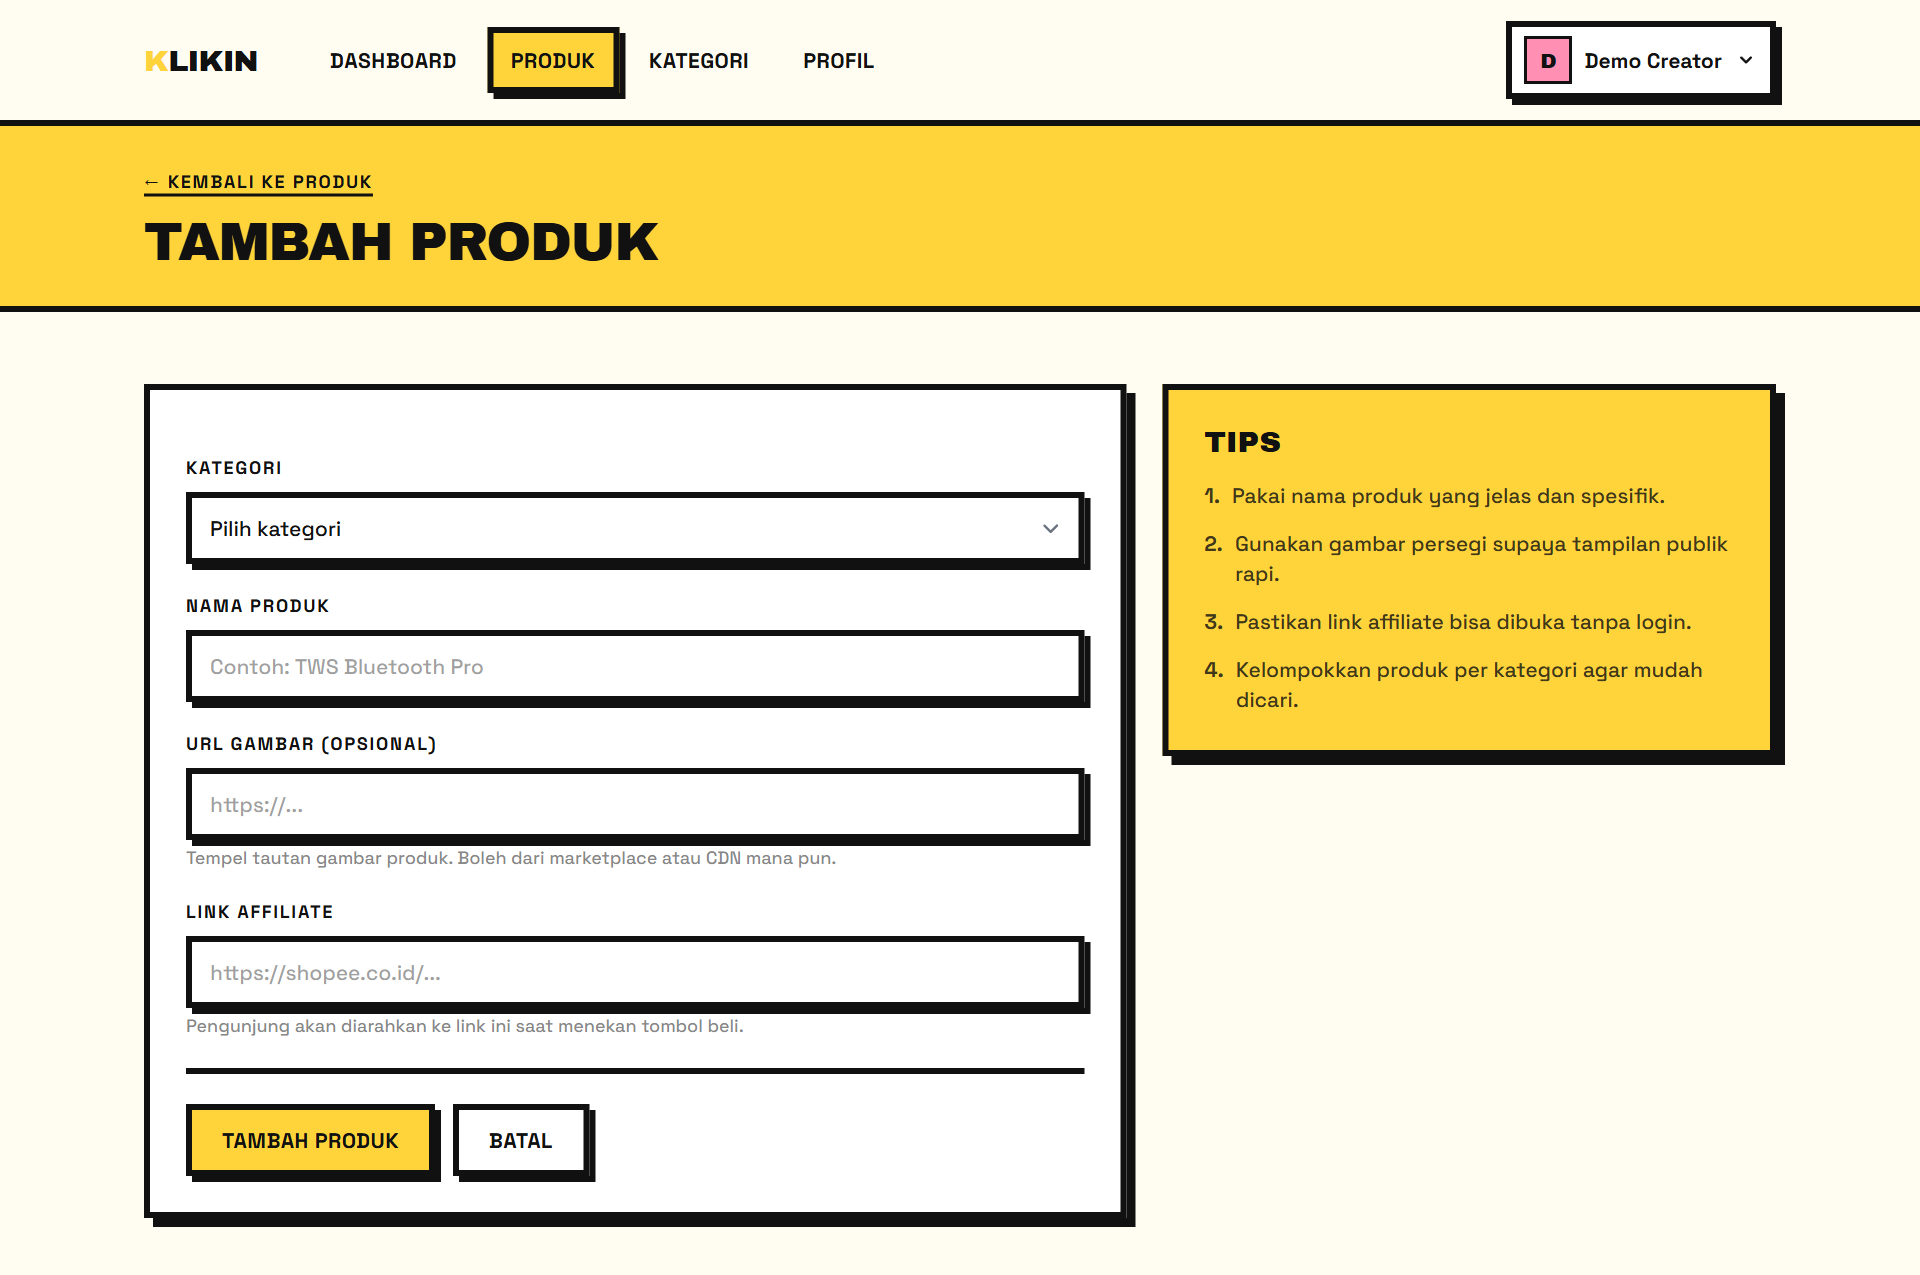
\includegraphics[width=\textwidth]{images/06_user_product_create.png}
        \caption{Formulir Tambah Produk Baru}
    \end{subfigure}
    \caption{Fitur Manajemen Produk Afiliasi}
    \label{fig:products}
\end{figure}

\newpage
\subsection{Manajemen Kategori \& Pengaturan Profil}
Kreator dapat menyusun kategori kustom agar etalase produk tersusun rapi, serta memperbarui bio, username, dan kata sandi akun mereka.
\begin{figure}[H]
    \centering
    \begin{subfigure}[b]{0.48\textwidth}
        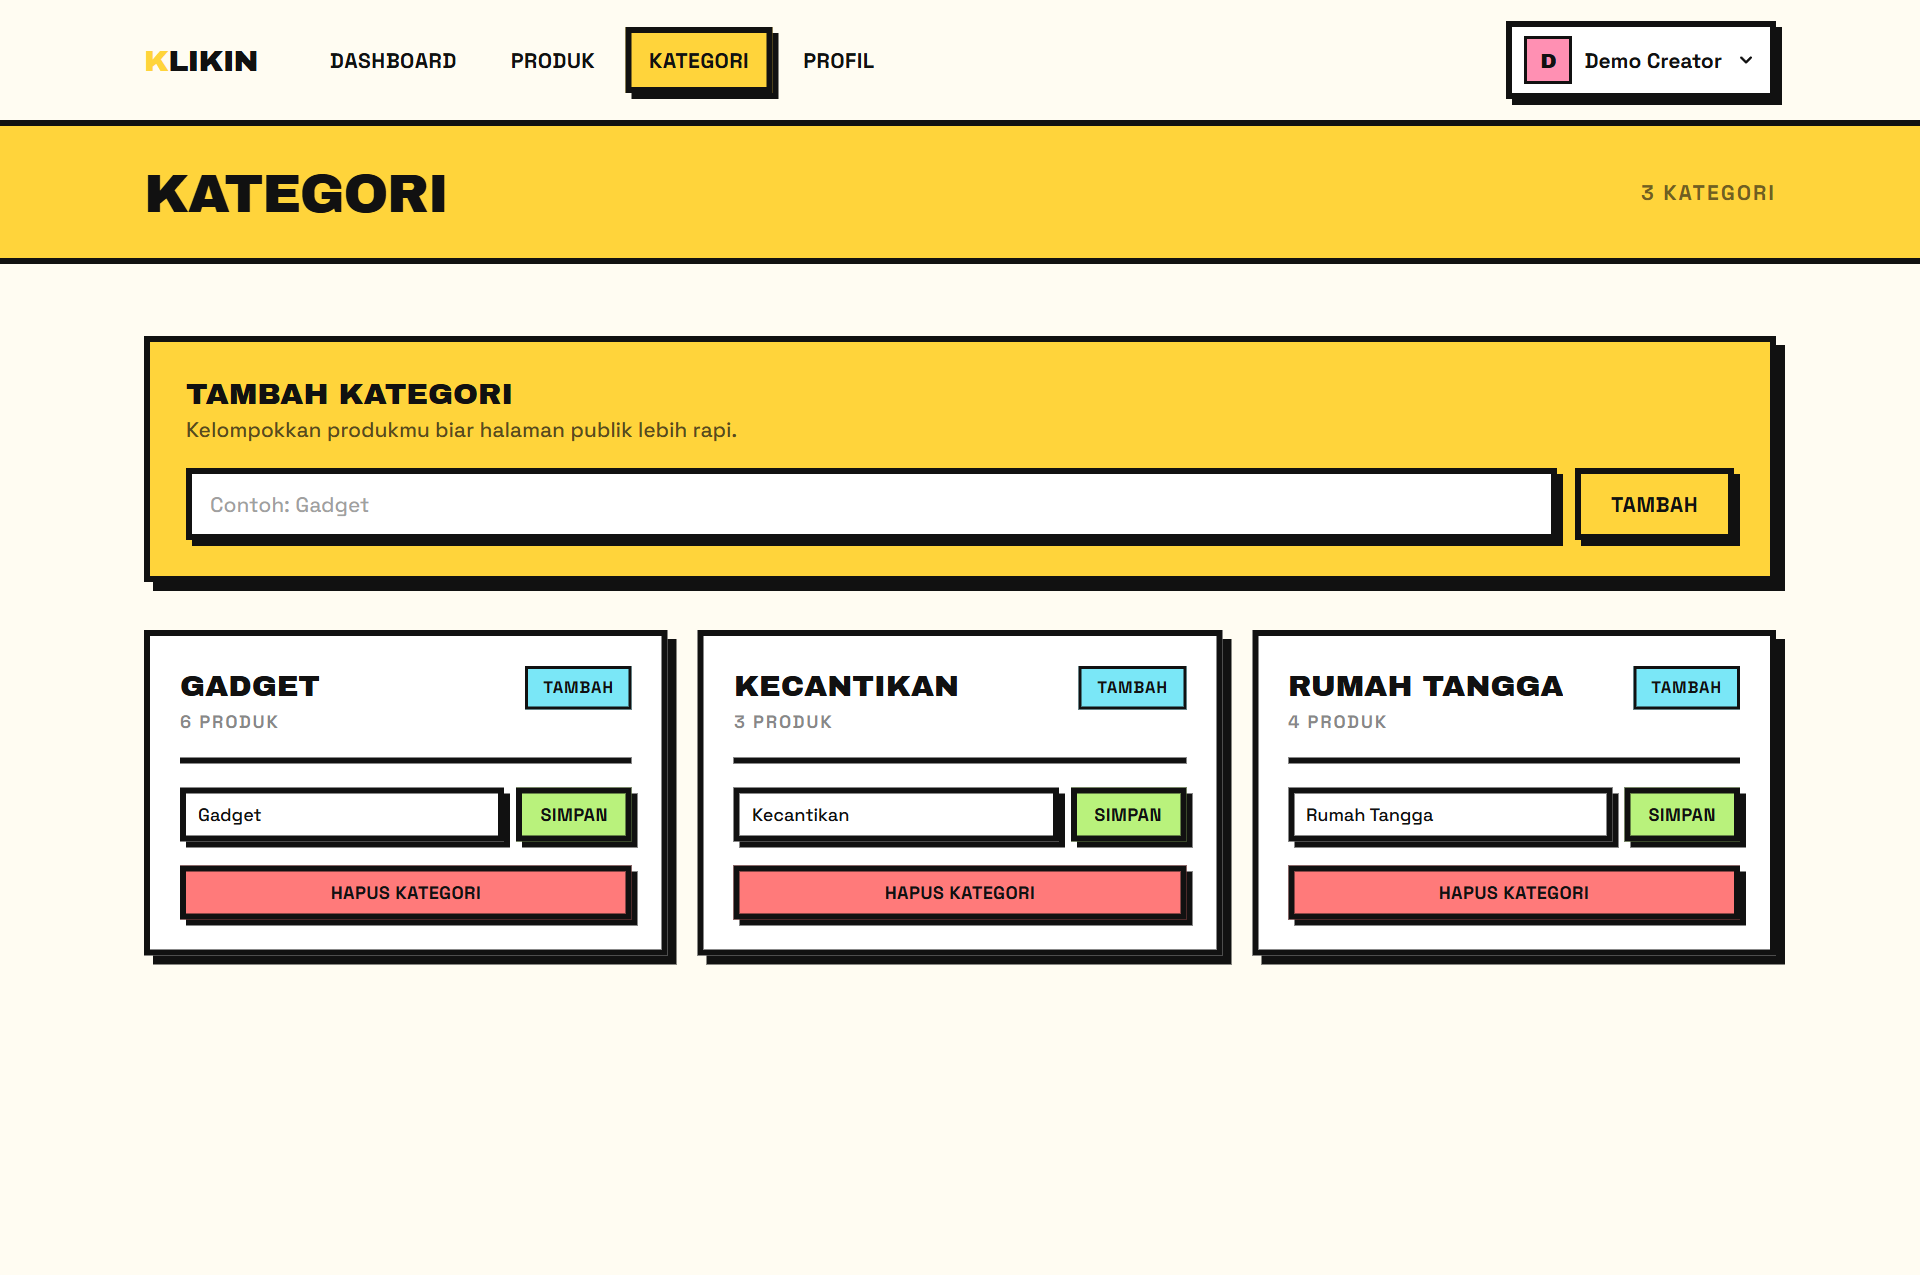
\includegraphics[width=\textwidth]{images/07_user_categories.png}
        \caption{Halaman Kelola Kategori}
    \end{subfigure}
    \hfill
    \begin{subfigure}[b]{0.48\textwidth}
        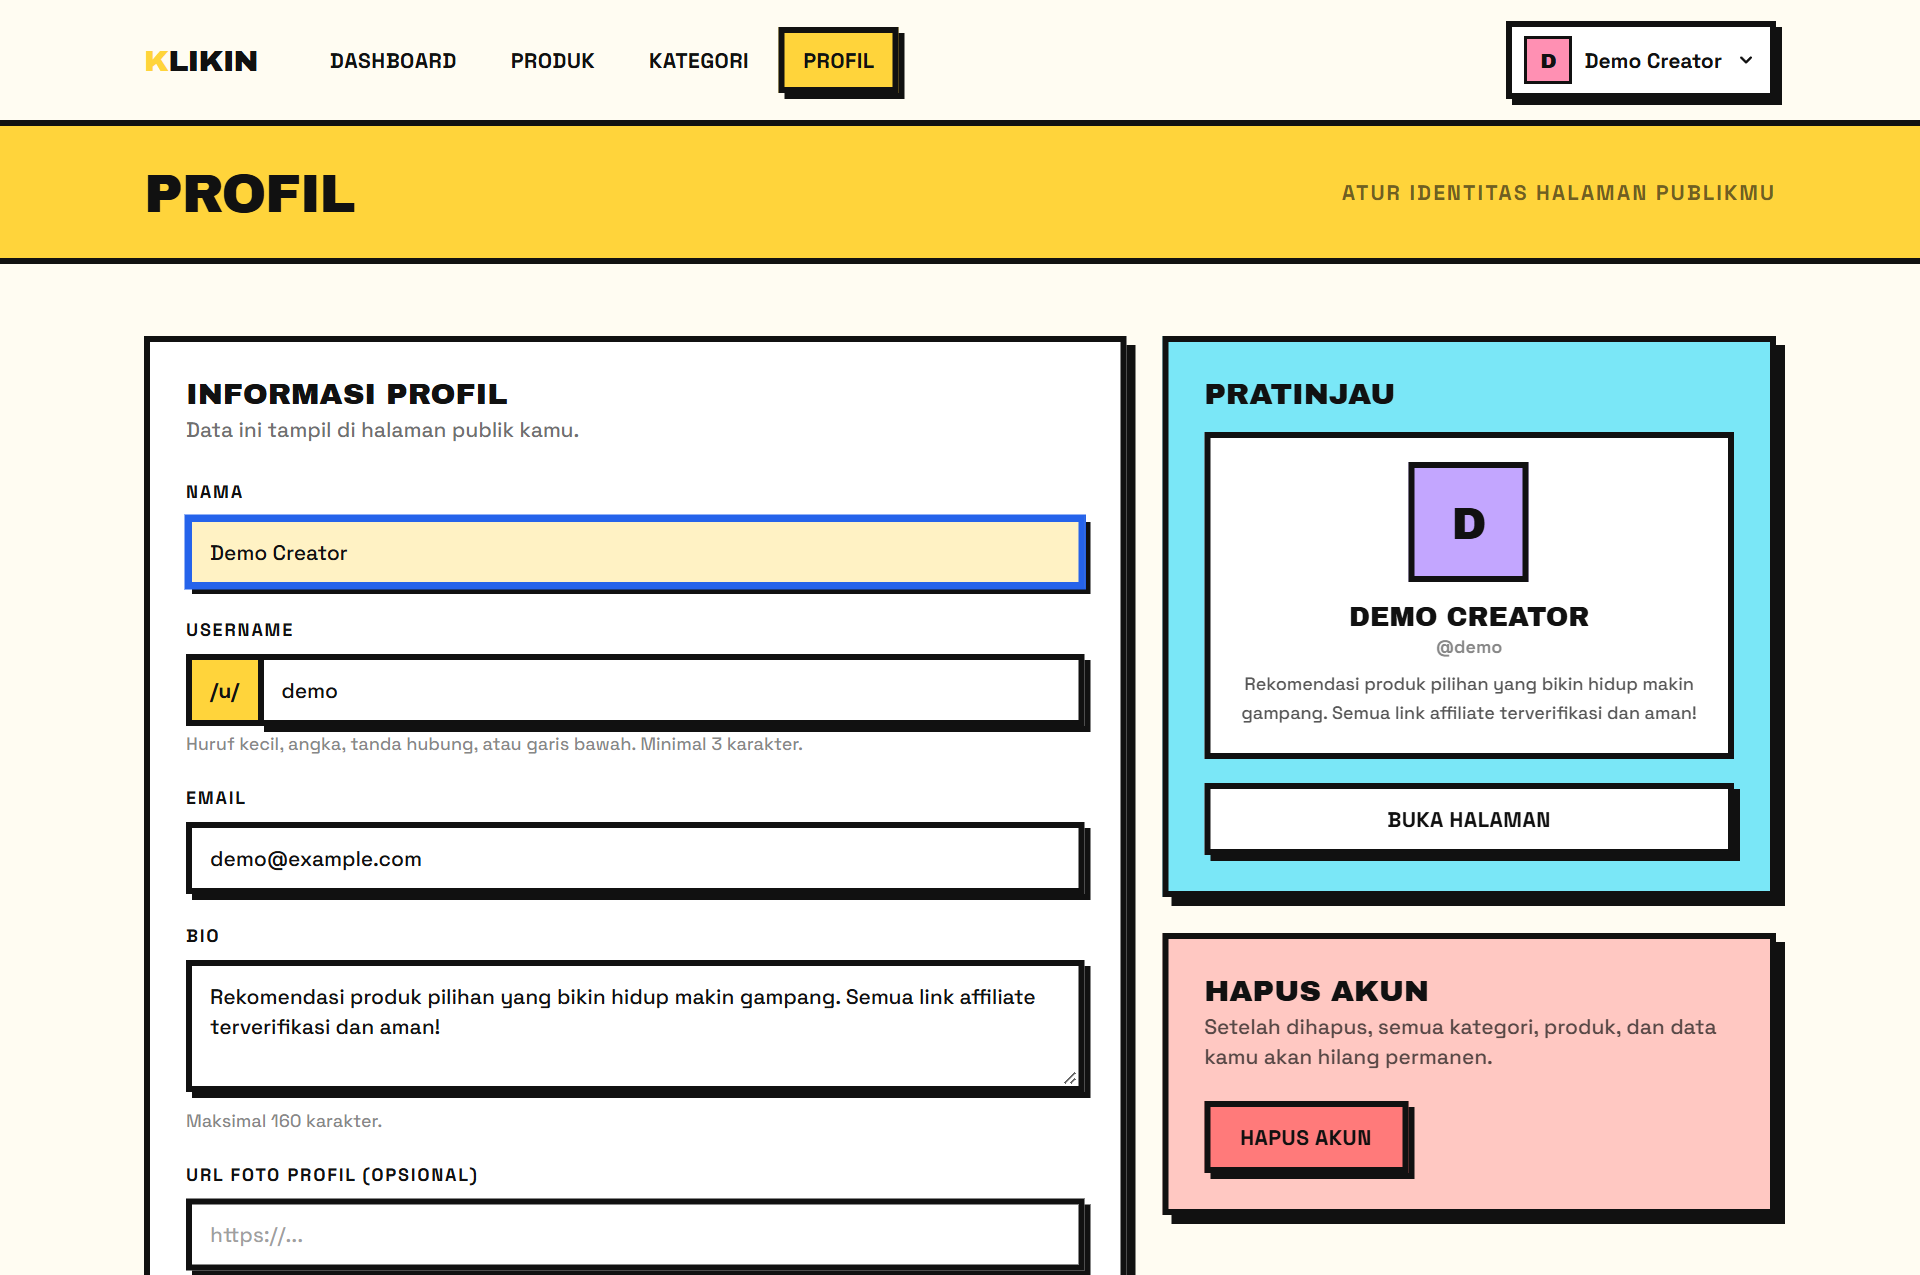
\includegraphics[width=\textwidth]{images/08_user_profile_edit.png}
        \caption{Pengaturan Profil \& Akun}
    \end{subfigure}
    \caption{Pengelolaan Kategori dan Pengaturan Akun}
    \label{fig:category_profile}
\end{figure}

\subsection{Halaman Publik Profil Kreator Aktif}
Halaman yang diakses oleh pengikut kreator melalui tautan \texttt{/u/\{username\}}. Produk ditampilkan terkelompok rapi per kategori dengan fitur pencarian interaktif berbasis Alpine.js.
\begin{figure}[H]
    \centering
    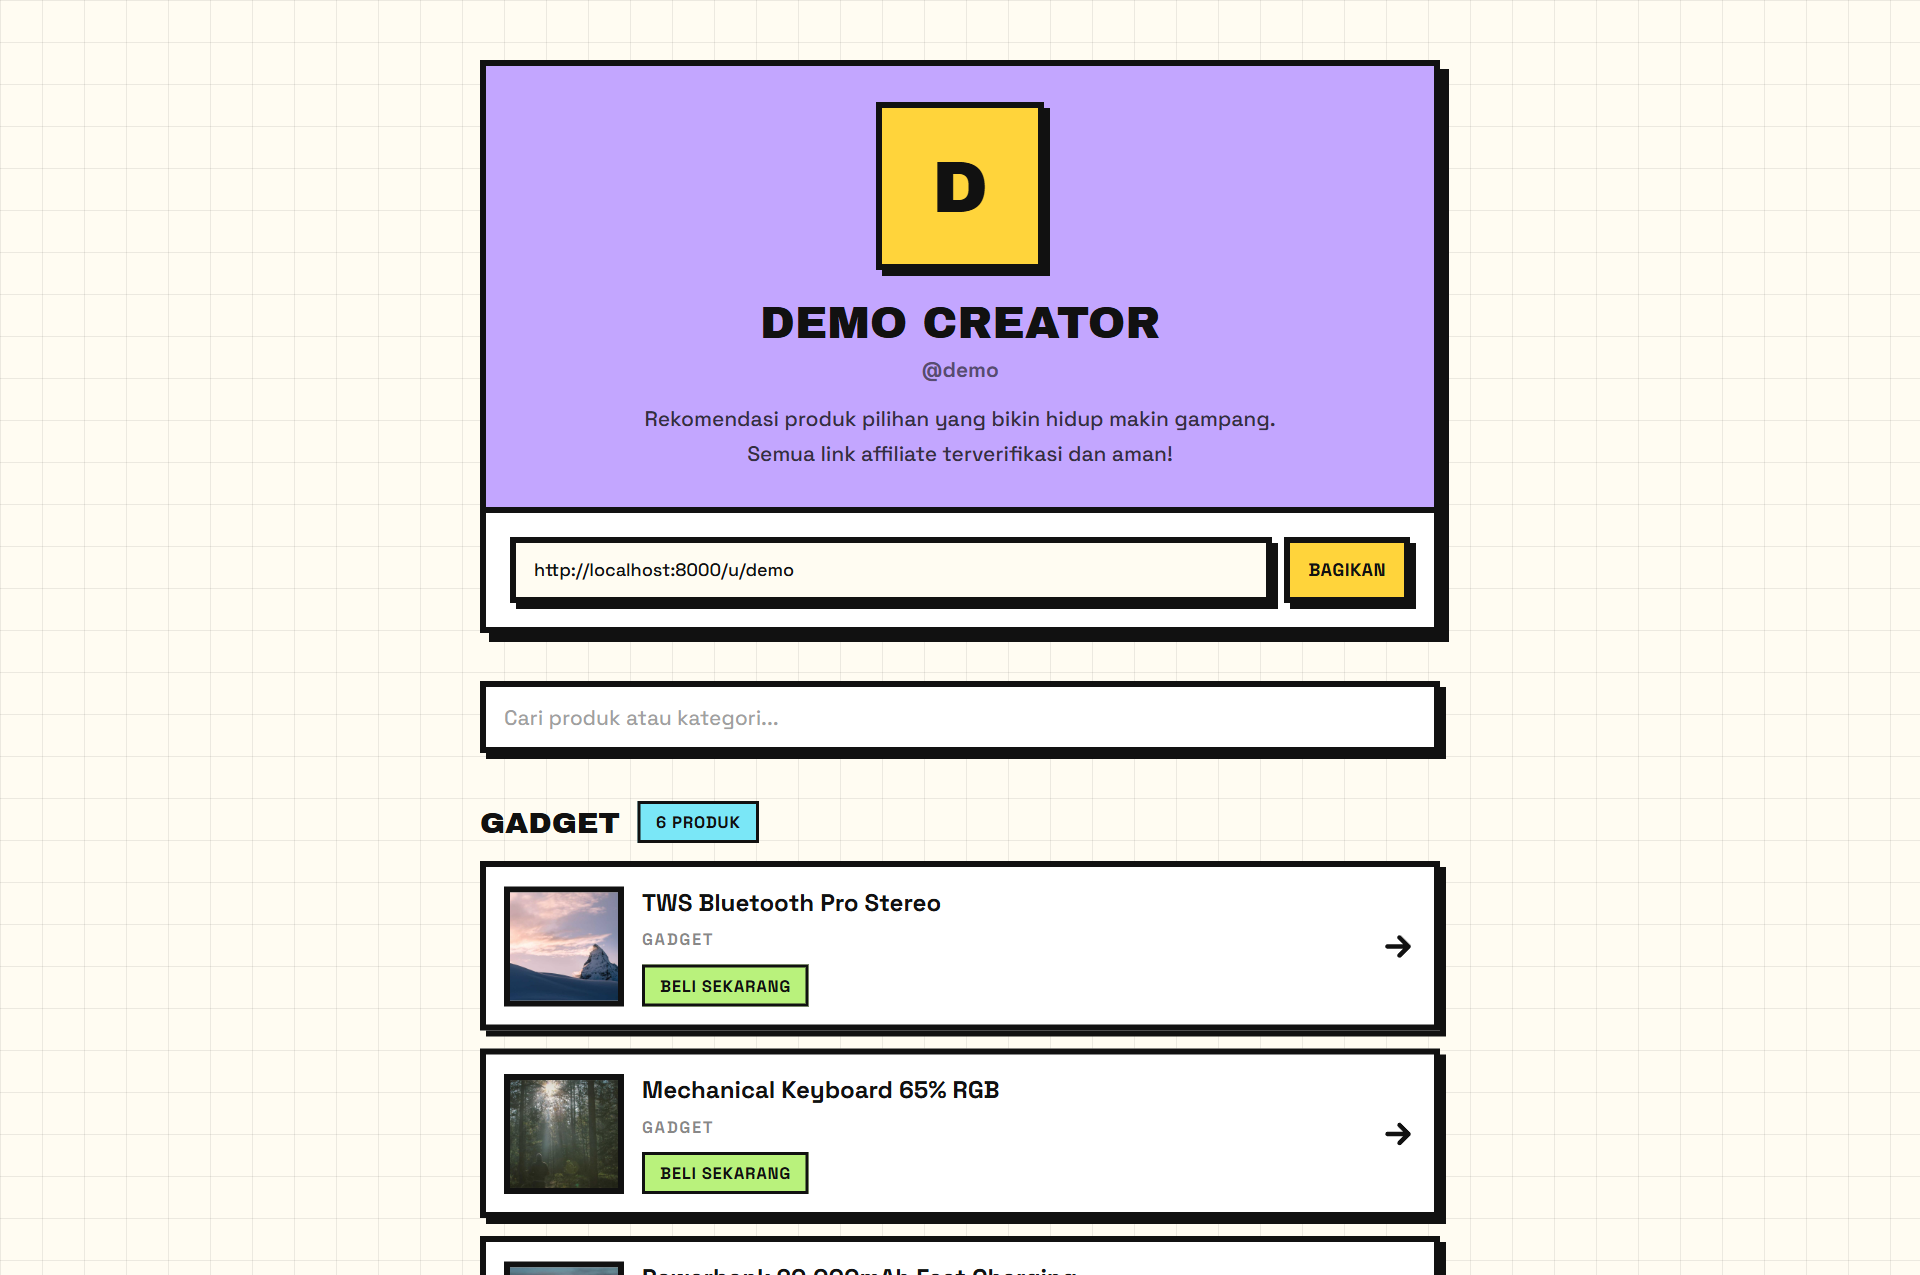
\includegraphics[width=0.88\textwidth]{images/09_public_profile_active.png}
    \caption{Halaman Publik Kreator Aktif (\texttt{/u/demo})}
    \label{fig:public_profile}
\end{figure}

\newpage
\subsection{Halaman Peringatan Pelanggaran Profil ``DO NOT CROSS''}
Inilah fitur inti penegakan aturan yang diminta. Ketika pengguna terbukti melanggar aturan dan di-\textit{ban} oleh Master, profil publiknya disegel secara visual dengan garis polisi dan alasan penindakan resmi.
\begin{figure}[H]
    \centering
    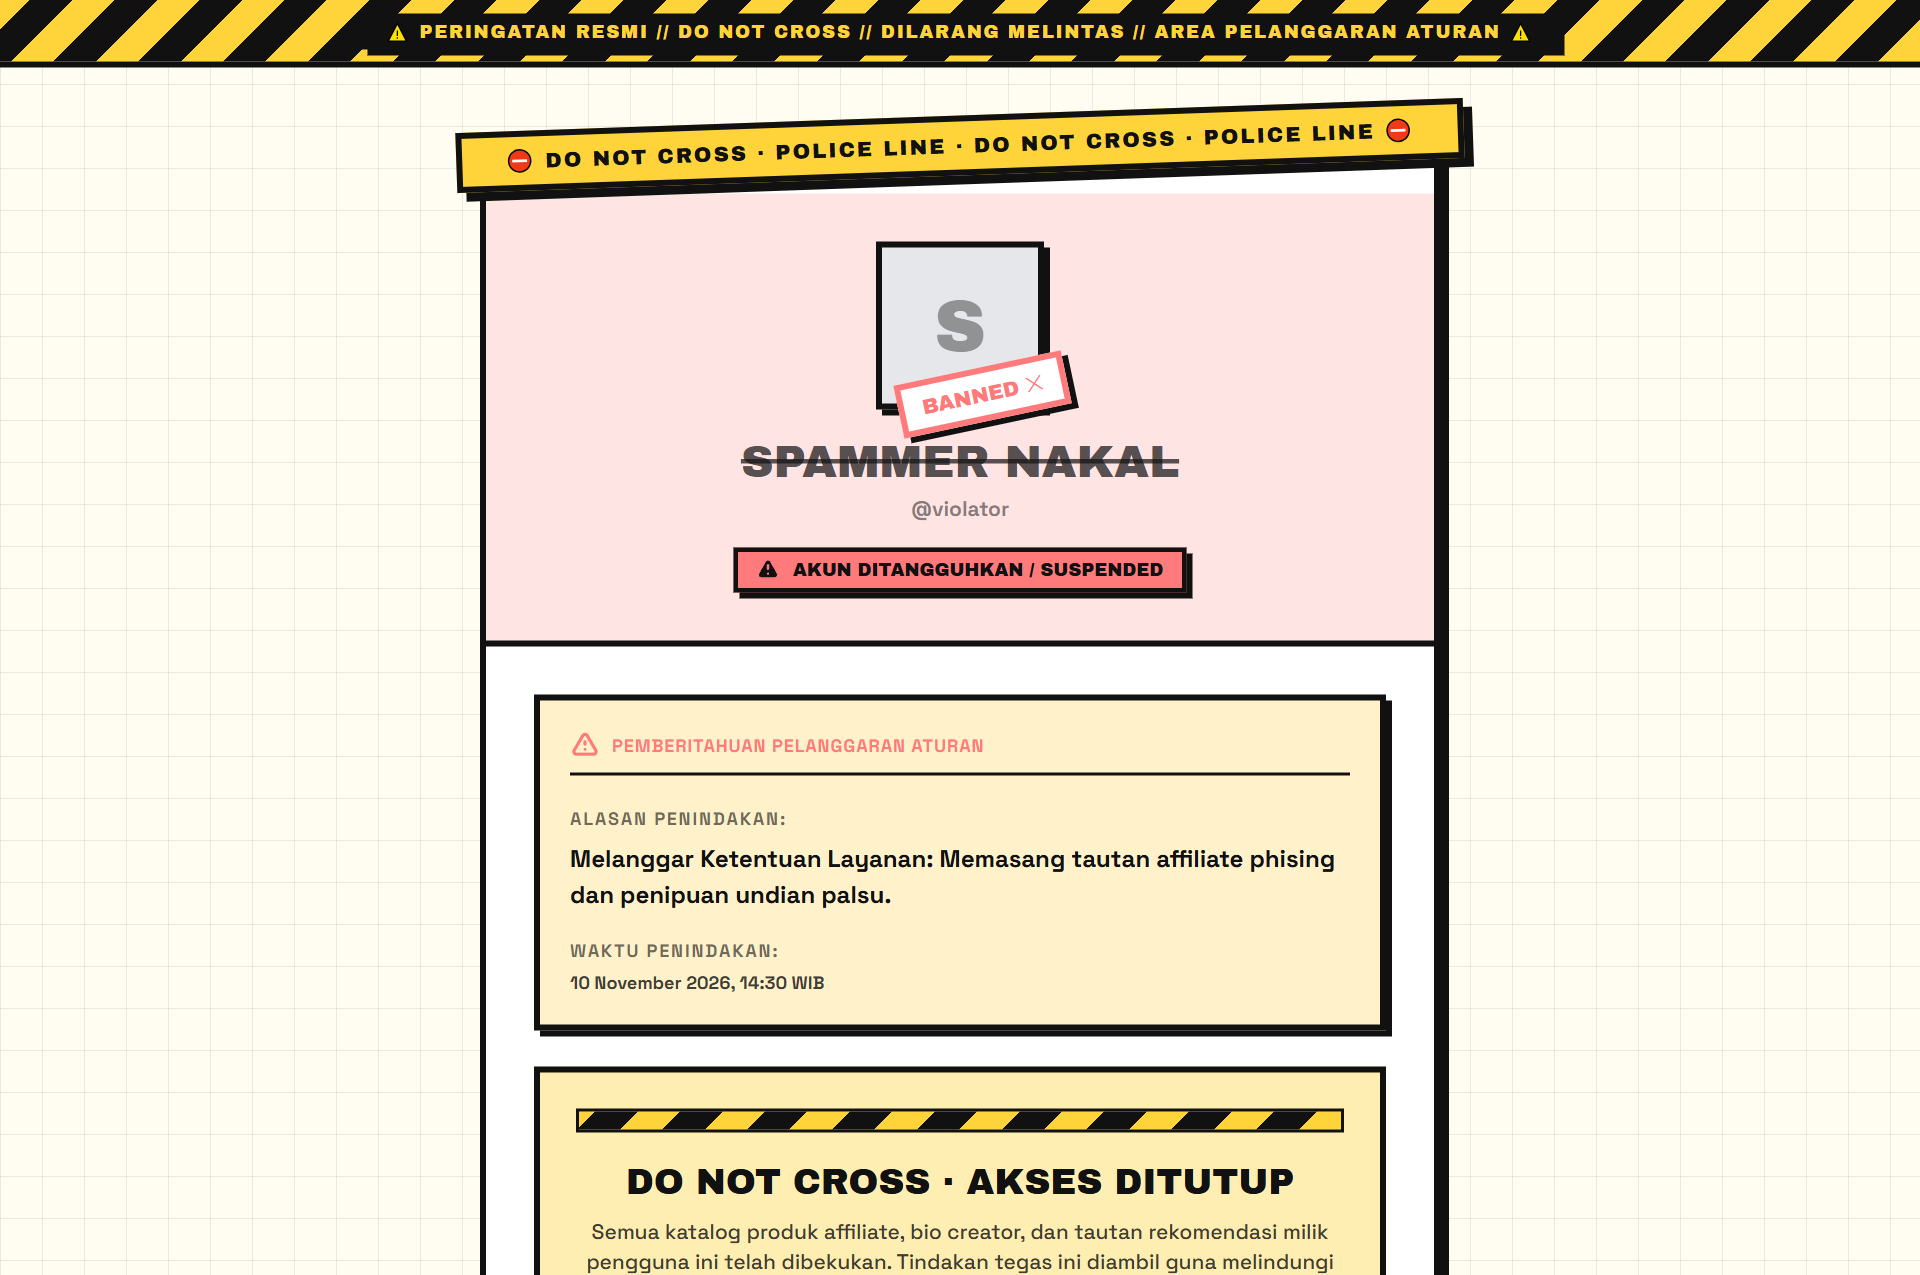
\includegraphics[width=0.92\textwidth]{images/10_public_profile_banned_donotcross.png}
    \caption{Tampilan Segel Pelanggaran DO NOT CROSS (\texttt{/u/violator})}
    \label{fig:banned_donotcross}
\end{figure}

\subsection{Dashboard Master Administrator}
Ketika login sebagai Master, pada bagian teratas dashboard muncul kartu otoritas khusus yang menandakan status Master Administrator dan menyediakan pintasan langsung ke Panel Pengguna.
\begin{figure}[H]
    \centering
    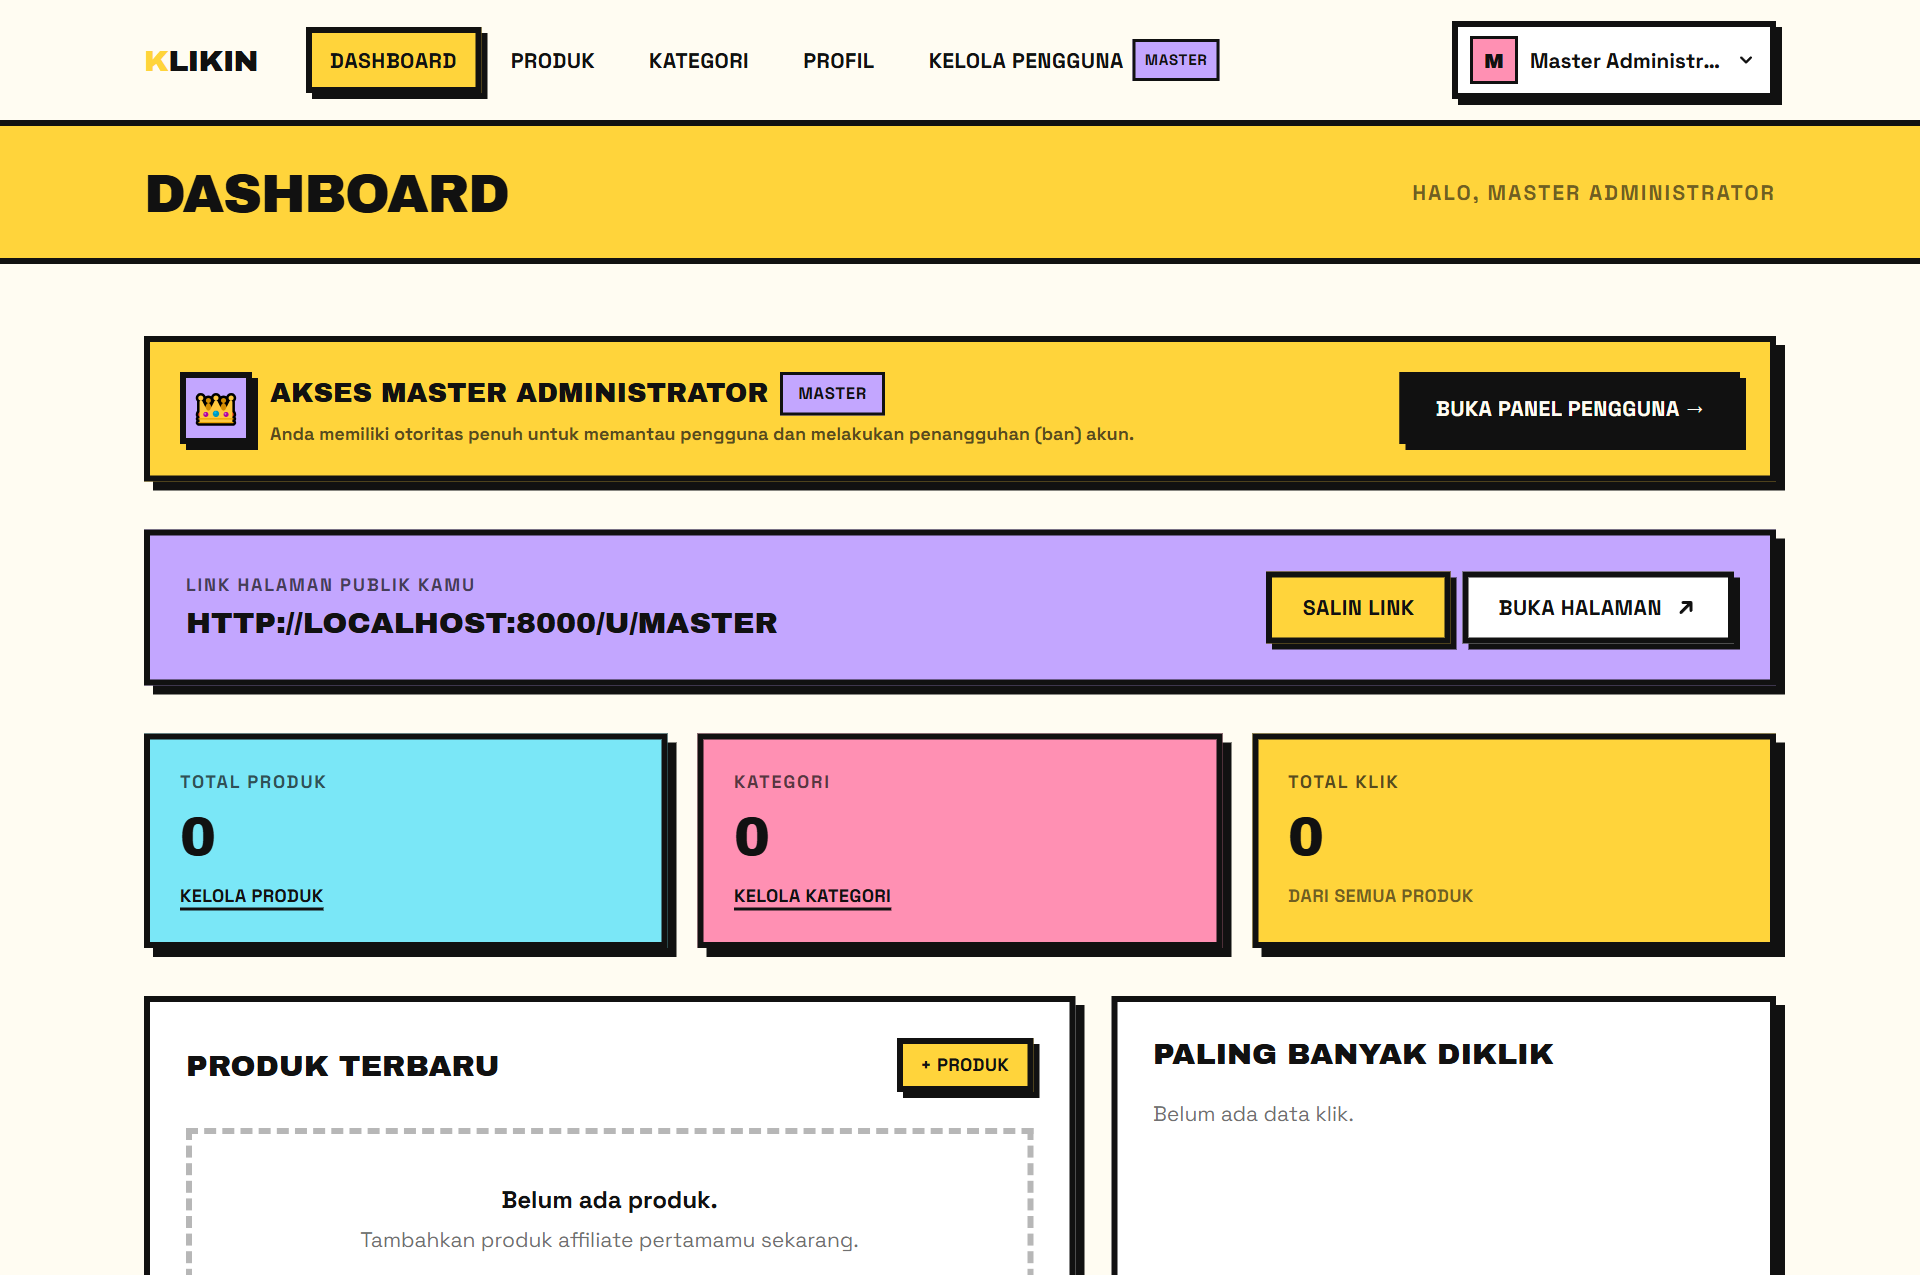
\includegraphics[width=0.92\textwidth]{images/11_master_dashboard.png}
    \caption{Dashboard dengan Notifikasi Akses Master Administrator}
    \label{fig:master_dashboard}
\end{figure}

\newpage
\subsection{Panel Kelola Pengguna Master (\texttt{/admin/users})}
Pusat kendali Master Administrator untuk memantau seluruh pengguna. Dilengkapi kartu statistik pengguna, filter berdasarkan Role (Semua, Master, User), filter Status (Aktif, Banned), kotak pencarian, serta tombol aksi penindakan.
\begin{figure}[H]
    \centering
    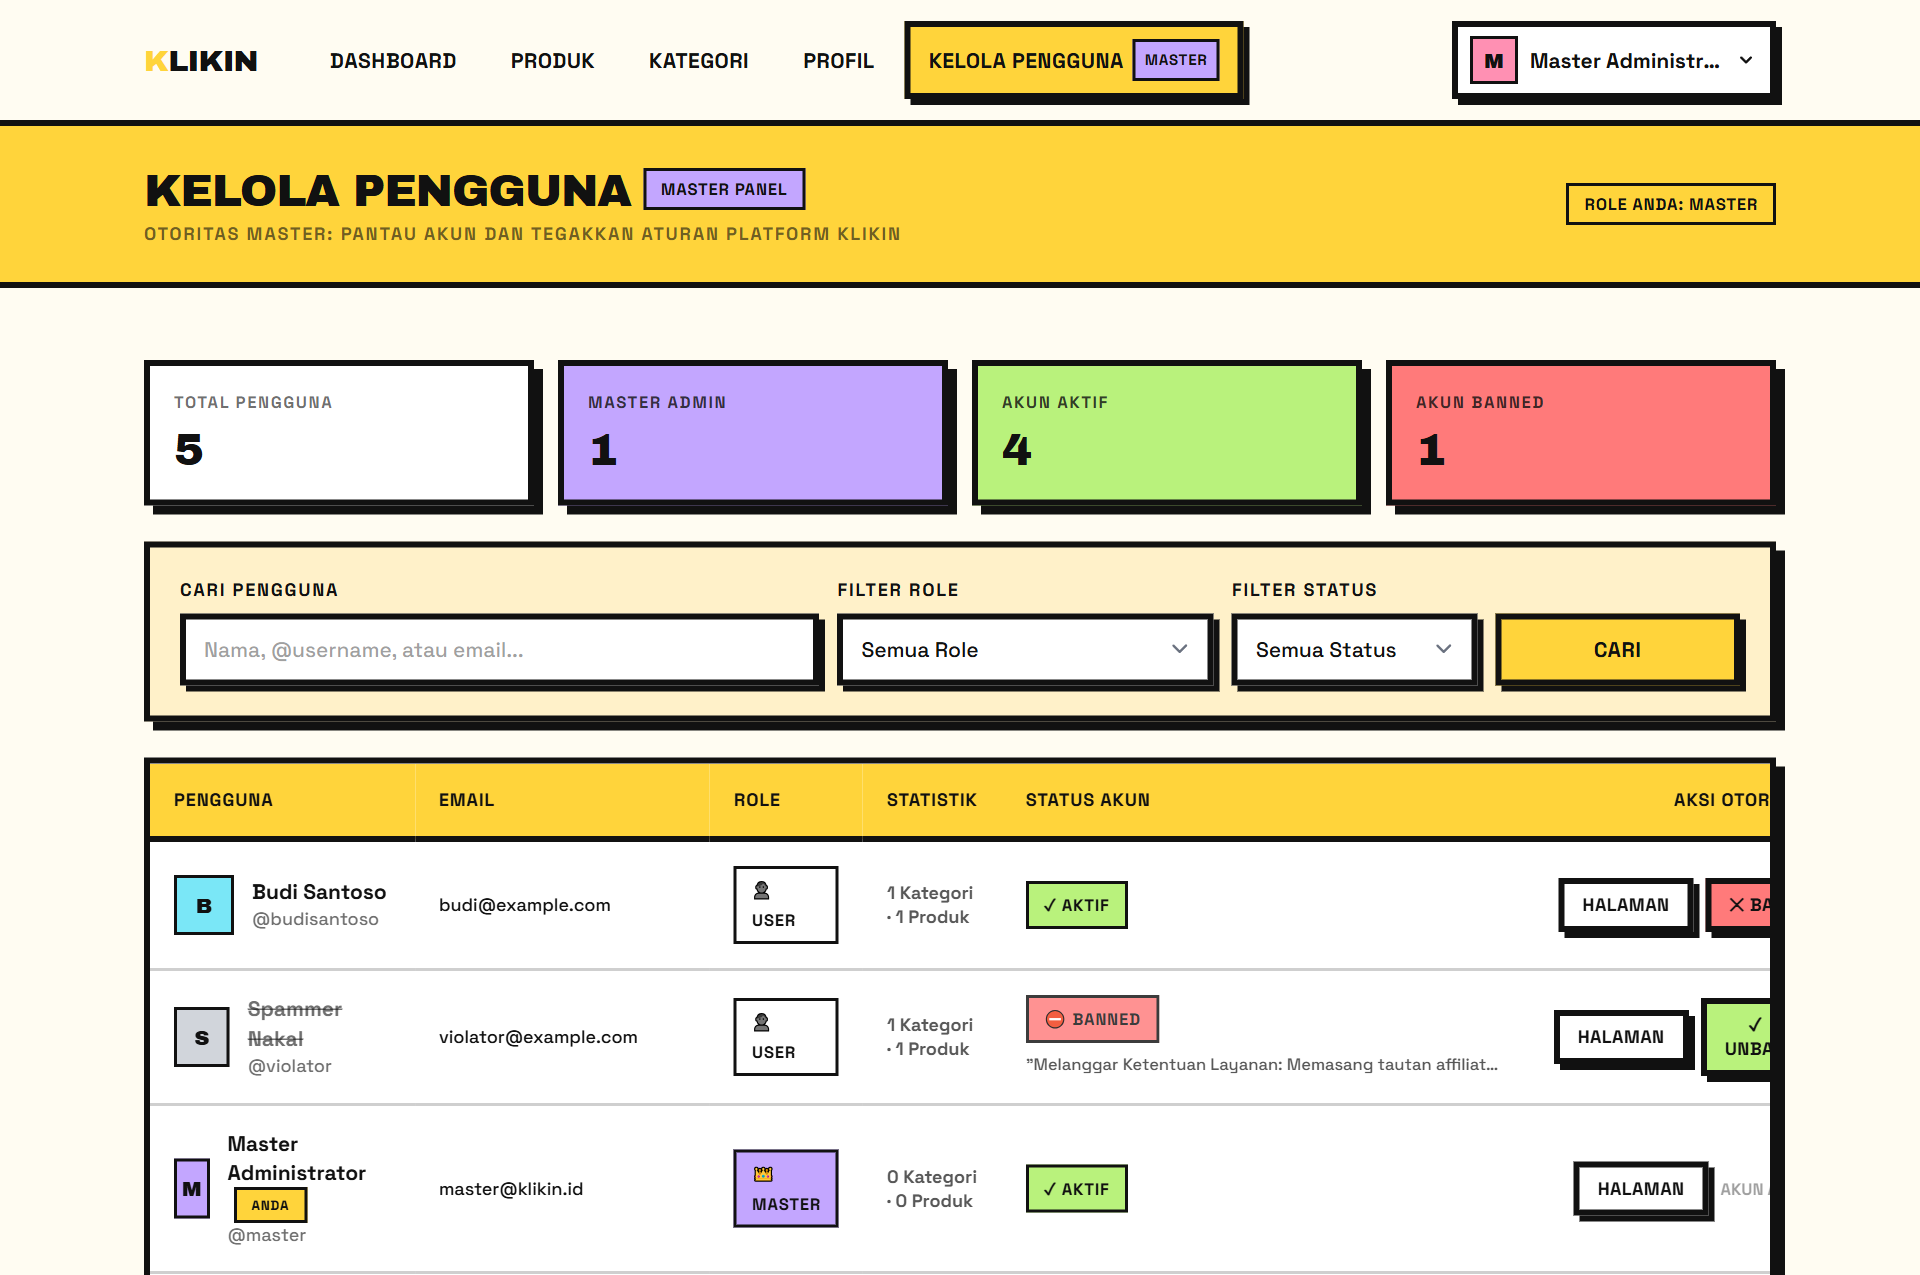
\includegraphics[width=0.92\textwidth]{images/12_master_users_panel.png}
    \caption{Panel Kelola Pengguna Master Administrator}
    \label{fig:master_users}
\end{figure}

\subsection{Modal Penindakan Ban \& Aksi Otoritas}
Master dapat menekan tombol ``[X] Ban'' pada baris pengguna tertentu untuk membuka modal dialog interaktif, mengisikan alasan penindakan, dan memproses penangguhan akun.
\begin{figure}[H]
    \centering
    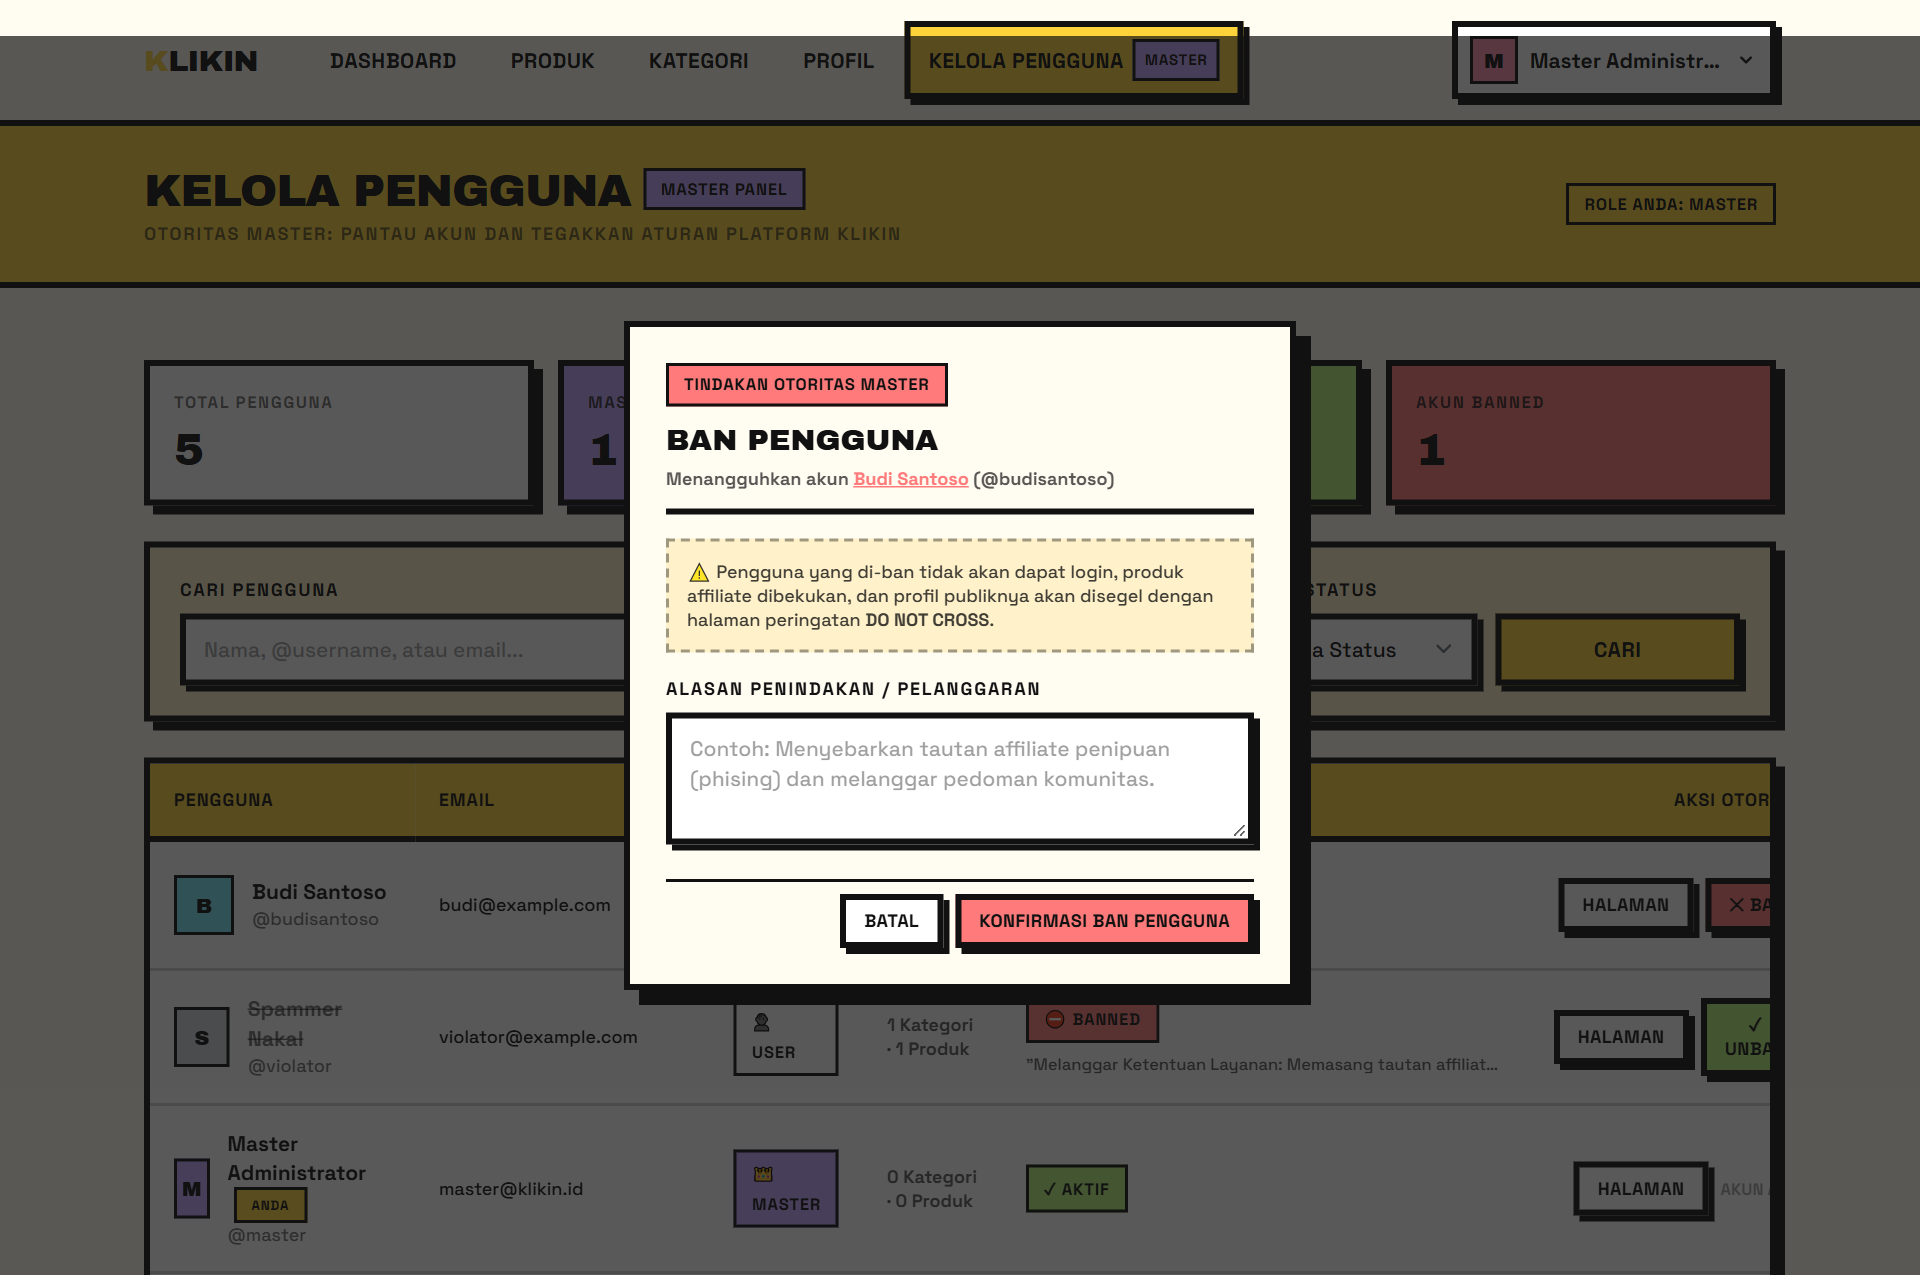
\includegraphics[width=0.90\textwidth]{images/13_master_ban_modal.png}
    \caption{Modal Dialog Penindakan Ban dengan Input Alasan Pelanggaran}
    \label{fig:ban_modal}
\end{figure}

\newpage
\subsection{Pengawasan Profil Banned oleh Master}
Jika Master membuka profil yang sedang di-\textit{ban}, sistem secara otomatis menyematkan bilah kendali (\textit{Master Control Bar}) di bagian atas dengan tombol instan untuk memulihkan akun (\textit{Unban Pengguna Ini}).
\begin{figure}[H]
    \centering
    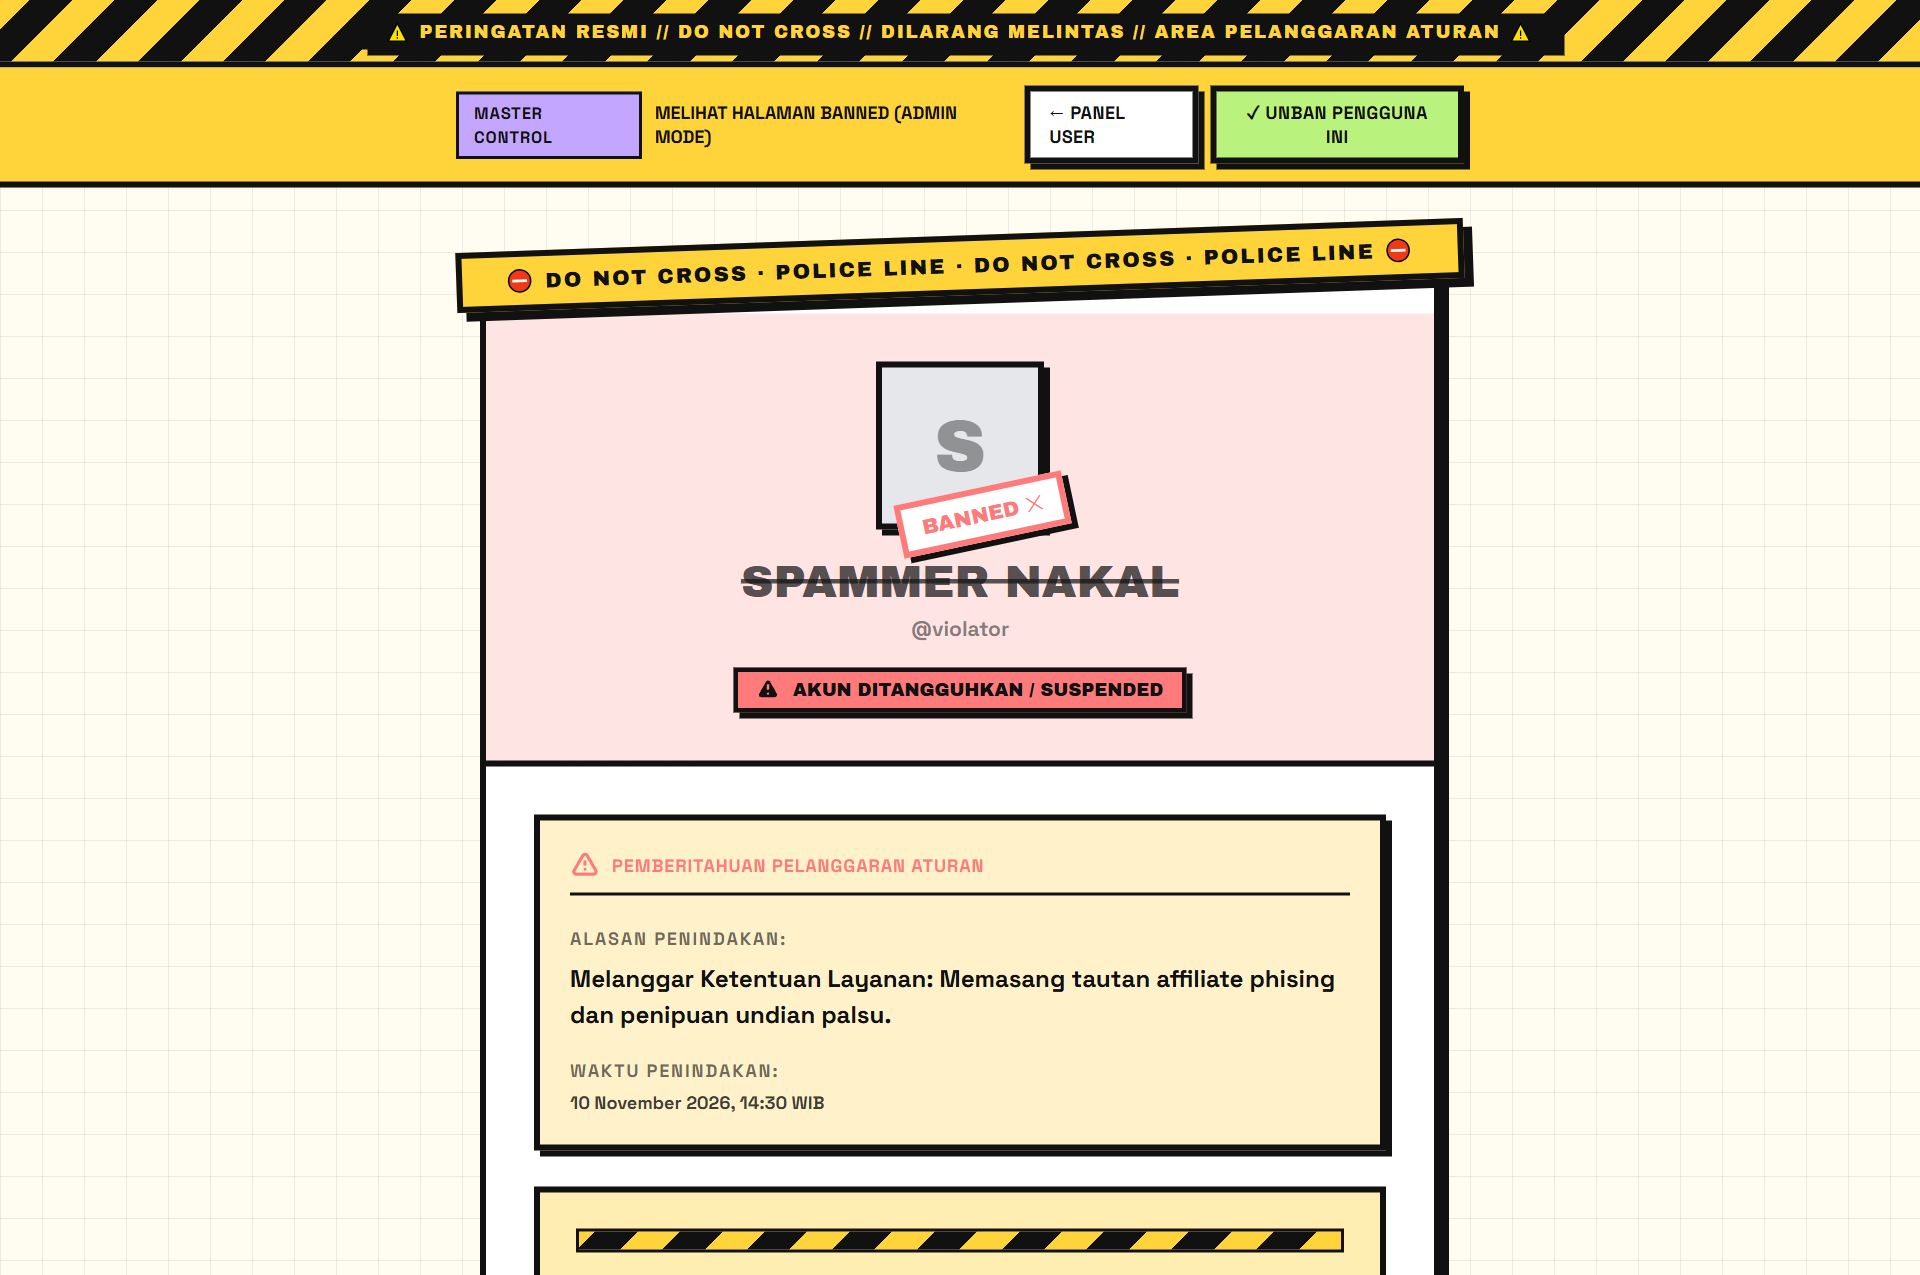
\includegraphics[width=0.90\textwidth]{images/14_master_view_banned_profile.png}
    \caption{Master Control Bar pada Halaman Profil Banned}
    \label{fig:master_view_banned}
\end{figure}

\subsection{Penolakan Login Otomatis Akun Ter-ban}
Apabila pengguna yang akunnya telah ditangguhkan mencoba untuk masuk, sistem secara otomatis menolak autentikasi dan memunculkan pesan peringatan resmi beserta alasan penindakan yang diberikan oleh Master.
\begin{figure}[H]
    \centering
    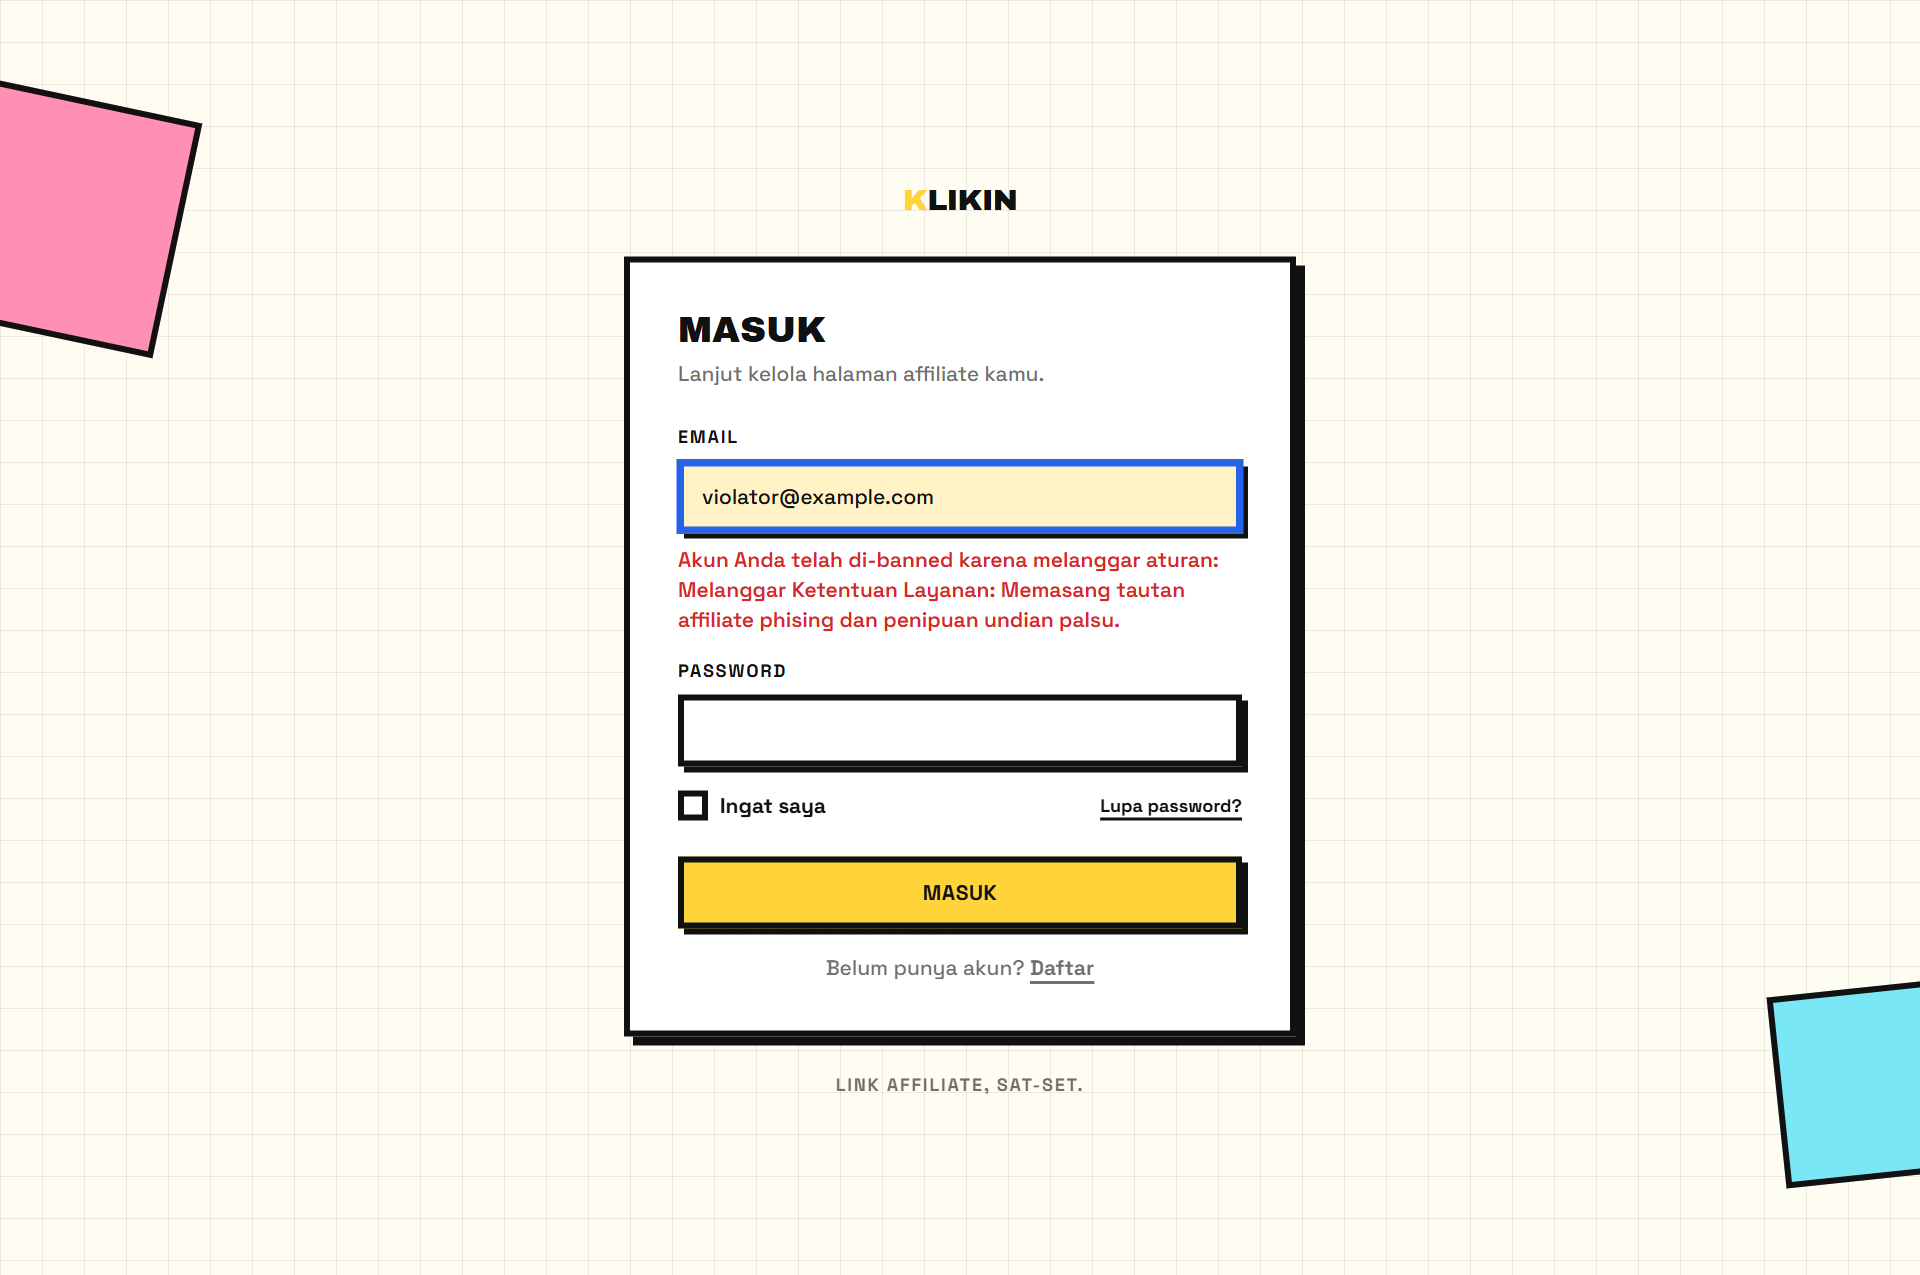
\includegraphics[width=0.75\textwidth]{images/15_banned_login_attempt.png}
    \caption{Pesan Penolakan Login Otomatis untuk Akun Banned}
    \label{fig:banned_login}
\end{figure}

\newpage

% ========================================================
% BAB 5: LAPORAN PENGUJIAN SISTEM (TESTING)
% ========================================================
\section{Laporan Hasil Pengujian Sistem (Testing)}

\subsection{Metodologi Pengujian}
Pengujian sistem dilakukan dengan pendekatan \textit{Automated Testing} menggunakan \textbf{Pest PHP 5}. Pengujian mencakup dua tingkat:
\begin{enumerate}[noitemsep]
    \item \textbf{Unit Testing}: Pengujian logika model internal, metode \textit{helper}, dan aturan validasi.
    \item \textbf{Feature Testing}: Pengujian aliran HTTP terintegrasi, middleware otoritas, sesi, penanganan basis data, hingga pengalihan halaman.
\end{enumerate}

\subsection{Hasil Eksekusi Test Suite}
Pengujian otomatis dijalankan pada seluruh test suite aplikasi melalui perintah:
\begin{lstlisting}[language=bash]
php artisan test --compact
\end{lstlisting}

\begin{tcolorbox}[
    colback=nbLime!20,
    colframe=nbInk,
    boxrule=2pt,
    arc=0mm,
    title={\bfseries RINGKASAN EKSEKUSI PEST TESTING}
]
\textbf{Total Pengujian (Tests)} : 48 Passed (100\% Berhasil) \\
\textbf{Total Pernyataan (Assertions)} : 146 Assertions \\
\textbf{Status Eksekusi} : \textcolor{green!60!black}{\textbf{PASSED / GREEN (Tanpa Error)}} \\
\textbf{Waktu Eksekusi} : 6.09 Detik
\end{tcolorbox}

\subsection{Rincian Kasus Uji (Test Cases)}
Tabel berikut merangkum seluruh skenario pengujian yang telah dirancang dan dieksekusi:

\begin{longtable}{p{0.5cm}p{6.8cm}p{4.5cm}c}
\caption{Daftar Hasil Pengujian Fitur Otomatis} \label{tab:tests} \\
\toprule
\textbf{No} & \textbf{Skenario Pengujian} & \textbf{Berkas Test} & \textbf{Hasil} \\
\midrule
\endfirsthead
\toprule
\textbf{No} & \textbf{Skenario Pengujian} & \textbf{Berkas Test} & \textbf{Hasil} \\
\midrule
\endhead
\bottomrule
\endfoot
1 & Helper role \texttt{isMaster()} \& \texttt{isUser()} & \texttt{MasterRoleAndBanTest} & \textbf{PASS} \\
2 & Tamu (Guest) dilarang akses panel user & \texttt{MasterRoleAndBanTest} & \textbf{PASS} \\
3 & User biasa dilarang akses panel user (403) & \texttt{MasterRoleAndBanTest} & \textbf{PASS} \\
4 & Master berhasil akses panel dan melihat daftar user & \texttt{MasterRoleAndBanTest} & \textbf{PASS} \\
5 & Master berhasil mem-ban user reguler & \texttt{MasterRoleAndBanTest} & \textbf{PASS} \\
6 & Master tidak dapat mem-ban akunnya sendiri & \texttt{MasterRoleAndBanTest} & \textbf{PASS} \\
7 & Master tidak dapat mem-ban sesama Master & \texttt{MasterRoleAndBanTest} & \textbf{PASS} \\
8 & User biasa dilarang mem-ban user lain & \texttt{MasterRoleAndBanTest} & \textbf{PASS} \\
9 & Master berhasil memulihkan (\textit{unban}) user & \texttt{MasterRoleAndBanTest} & \textbf{PASS} \\
10 & User banned tidak bisa login \& melihat alasan & \texttt{BannedUserEnforcementTest} & \textbf{PASS} \\
11 & Profil banned menampilkan DO NOT CROSS & \texttt{BannedUserEnforcementTest} & \textbf{PASS} \\
12 & Profil banned menyembunyikan katalog produk & \texttt{BannedUserEnforcementTest} & \textbf{PASS} \\
13 & Profil user aktif menampilkan katalog normal & \texttt{BannedUserEnforcementTest} & \textbf{PASS} \\
14 & Redirect link affiliate diblokir jika user banned & \texttt{BannedUserEnforcementTest} & \textbf{PASS} \\
15 & Redirect link affiliate sukses jika user aktif & \texttt{BannedUserEnforcementTest} & \textbf{PASS} \\
16 & Middleware otomatis logout user aktif yang di-ban & \texttt{BannedUserEnforcementTest} & \textbf{PASS} \\
17 & Pengguna dapat melihat daftar produk miliknya & \texttt{AffiliateProductTest} & \textbf{PASS} \\
18 & Pengguna dapat menambah produk baru & \texttt{AffiliateProductTest} & \textbf{PASS} \\
19 & Pengguna dapat memperbarui produk miliknya & \texttt{AffiliateProductTest} & \textbf{PASS} \\
20 & Pengguna dapat menghapus produk miliknya & \texttt{AffiliateProductTest} & \textbf{PASS} \\
21 & Pengguna dilarang menyunting produk orang lain & \texttt{AffiliateProductTest} & \textbf{PASS} \\
22 & Pengguna dilarang menghapus produk orang lain & \texttt{AffiliateProductTest} & \textbf{PASS} \\
23 & Tautan redirect menambah hitungan klik (+1) & \texttt{AffiliateProductTest} & \textbf{PASS} \\
24 & Halaman profil dapat diakses pengguna & \texttt{ProfileTest} & \textbf{PASS} \\
25 & Informasi profil dapat diperbarui & \texttt{ProfileTest} & \textbf{PASS} \\
26 & Status verifikasi email tidak berubah jika email sama & \texttt{ProfileTest} & \textbf{PASS} \\
27 & Pengguna dapat menghapus akunnya sendiri & \texttt{ProfileTest} & \textbf{PASS} \\
28 & Sandi salah mencegah penghapusan akun & \texttt{ProfileTest} & \textbf{PASS} \\
29 & Layar login dapat ditampilkan & \texttt{Auth\textbackslash AuthenticationTest} & \textbf{PASS} \\
30 & Pengguna dapat login dengan sandi benar & \texttt{Auth\textbackslash AuthenticationTest} & \textbf{PASS} \\
31 & Pengguna gagal login dengan sandi salah & \texttt{Auth\textbackslash AuthenticationTest} & \textbf{PASS} \\
32 & Pengguna dapat logout dari aplikasi & \texttt{Auth\textbackslash AuthenticationTest} & \textbf{PASS} \\
33 & Layar registrasi dapat ditampilkan & \texttt{Auth\textbackslash RegistrationTest} & \textbf{PASS} \\
34 & Pengguna baru berhasil terdaftar di database & \texttt{Auth\textbackslash RegistrationTest} & \textbf{PASS} \\
35-48 & Uji Verifikasi Email, Reset Sandi, \& Konfirmasi & Berkas Auth Lainnya & \textbf{PASS} \\
\end{longtable}

\newpage

% ========================================================
% BAB 6: KESIMPULAN & PENUTUP
% ========================================================
\section{Kesimpulan}

Berdasarkan seluruh tahapan perancangan, implementasi fitur, dan pengujian sistem yang telah dilakukan, dapat diambil beberapa kesimpulan:
\begin{enumerate}
    \item \textbf{Implementasi Role Master \& User}: Sistem berhasil memisahkan wewenang antara pengguna biasa (\textit{user}) dan pengelola (\textit{master}) dengan rapi melalui penambahan kolom pada basis data serta penyematan middleware \texttt{EnsureUserIsMaster}.
    \item \textbf{Fitur Penangguhan (Ban) \& Halaman DO NOT CROSS}: Fitur ban berfungsi secara menyeluruh mulai dari penolakan login, pemutusan sesi aktif secara otomatis, proteksi tautan \textit{redirect}, hingga penutupan konten profil publik kreator dengan tampilan visual barikade \textit{Police Line DO NOT CROSS} yang sangat informatif dan mematuhi estetika desain Neobrutalism.
    \item \textbf{Penyediaan Seeder Otomatis}: Berkas seeder \texttt{MasterSeeder} dan \texttt{UserSeeder} telah dikonfigurasi untuk memudahkan inisialisasi akun Master Administrator, kreator reguler, dan akun pelanggar ter-\textit{ban} sebagai data uji coba.
    \item \textbf{Kualitas \& Keandalan Perangkat Lunak}: Seluruh pengujian fitur dan unit (sebanyak 48 skenario dengan 146 assertions) berhasil lulus 100\% tanpa kegagalan (\textit{all green}), membuktikan bahwa sistem memiliki keandalan tinggi dan bebas dari regresi.
\end{enumerate}

Dengan demikian, seluruh instruksi dan persyaratan tugas UAS Pemrograman Web 2 ini telah terpenuhi secara sempurna.

\end{document}

